%%%%%%%%%%%%%%%%%%%%%%%%%%%%%%%%%%%%%%%%%
% Masters/Doctoral Thesis 
% LaTeX Template
% Version 2.4 (22/11/16)
%
% This template has been downloaded from:
% http://www.LaTeXTemplates.com
%
% Version 2.x major modifications by:
% Vel (vel@latextemplates.com)
%
% This template is based on a template by:
% Steve Gunn (http://users.ecs.soton.ac.uk/srg/softwaretools/document/templates/)
% Sunil Patel (http://www.sunilpatel.co.uk/thesis-template/)
%
% Template license:
% CC BY-NC-simulated annealing 3.0 (http://creativecommons.org/licenses/by-nc-sa/3.0/)
%
%%%%%%%%%%%%%%%%%%%%%%%%%%%%%%%%%%%%%%%%%

%--------------------------------------------
%	PACKAGES AND OTHER DOCUMENT CONFIGURATIONS
%--------------------------------------------

\documentclass[
11pt, % The default document font size, options: 10pt, 11pt, 12pt
%oneside, % Two side (alternating margins) for binding by default, uncomment to switch to one side
english, % ngerman for German
singlespacing, % Single line spacing, alternatives: onehalfspacing or doublespacing
%draft, % Uncomment to enable draft mode (no pictures, no links, overfull hboxes indicated)
nolistspacing, % If the document is onehalfspacing or doublespacing, uncomment this to set spacing in lists to single
liststotoc, % Uncomment to add the list of figures/tables/etc to the table of contents
%toctotoc, % Uncomment to add the main table of contents to the table of contents
%parskip, % Uncomment to add space between paragraphs
%nohyperref, % Uncomment to not load the hyperref package
headsepline, % Uncomment to get a line under the header
%chapterinoneline, % Uncomment to place the chapter title next to the number on one line
%consistentlayout, % Uncomment to change the layout of the declaration, abstract and acknowledgements pages to match the default layout
]{MastersDoctoralThesis} % The class file specifying the document structure


% Imports
\usepackage{palatino} % Use the Palatino font by default

% Encoding
\usepackage[utf8]{inputenc} % Required for inputting international characters
\usepackage[T1]{fontenc} % Output font encoding for international characters

% Logical
\usepackage{xifthen}
\usepackage{ifdraft}

% Bilbliography
\usepackage[style=numeric,natbib=true,giveninits=true,sorting=none]{biblatex}

% Document class "MasterDoctoralThesis" internals
\usepackage[autostyle=true]{csquotes} % Required to generate language-dependent quotes in the bibliography
\usepackage{import}
\usepackage{tocbibind}

% Images
\usepackage{graphicx} % Permet l'insertion d'image (entre autres)
\usepackage{pict2e} % Pour faire des graphiques

% Tikz and colors
\usepackage{color}
\usepackage{xcolor}
\usepackage{tikz}
	\usetikzlibrary{arrows}
	\usetikzlibrary{calc}
	\usetikzlibrary{fadings}
	\usetikzlibrary{patterns}
	\usetikzlibrary{plotmarks}
	\usetikzlibrary{shapes}

% Maths
\usepackage{amsfonts} % Mathematical fonts
\usepackage{amsmath} % Mathematical environnements
\usepackage{amssymb} % Mathematical symbols
\usepackage{bbm}  % Extended blackboard bold symbols
\usepackage{mathrsfs}  % Super fancy script math fonts

% Tables and figures
\usepackage{array} % For tables
\usepackage{floatrow} % Customize floating environnement
\usepackage{subfig} % Subfigure possible
\usepackage{tabu} % Better tabular

% Misc
% \usepackage[english]{babel}  % Should not be used with MastersDoctoralThesis class
\usepackage[colorinlistoftodos, obeyFinal, color=black]{todonotes}
\usepackage{makeidx}  % allow to make an index
\usepackage{hyperref}
\usepackage{setspace}  % Allows to set line spacing and such
\usepackage{verbatim}  % Verbatim
\usepackage{xspace}  % Trailing space for custom commands

% Setup
\floatsetup[figure]{style=plain}
\hypersetup{
    colorlinks,
    linkcolor={red!50!black},
    citecolor={blue!50!black},
    urlcolor={blue!80!black}
}

% Labels and references
\ifoptionfinal{}{\usepackage{refcheck}}

% Dark theme
\makeatletter
\newcommand{\globalcolor}[1]{%
  \color{#1}\global\let\default@color\current@color
}
\makeatother

\ifoptionfinal{}
{
	\definecolor{darkbg}{HTML}{002b36}
	\definecolor{lighttext}{HTML}{93a1a1}

	\pagecolor{darkbg}
	\AtBeginDocument{\globalcolor{lighttext}}  % Change text color
}

% Symbols
\newcommand{\total}{\text{d}}  % d for total derivative

% Modifiers
\newcommand{\code}[1]{\texttt{#1}}  % shortcut to insert code inline
\newcommand{\myvec}[1]{\boldsymbol{\mathrm{#1}}}  % bold vectors

% Encompassing (i.e. somthing is put both side of the input}
\newcommand{\bigO}[1]{\mathcal{O}\!\left(#1\right)}  % big O notation
\newcommand{\expected}[2][]{\mathbb{E}_{#1}\!\left[ #2 \right]}
\newcommand{\interval}[1]{\left[#1\right]}
\newcommand{\norm}[1]{\Vert #1\Vert}  % norm of a vector
\newcommand{\set}[1]{\{#1\}}  % set notation with curly braces
\newcommand{\var}[1]{\mathrm{var}\!\left[ #1 \right]}
\newcommand{\todoi}[2][]{\todo[inline, #1]{#2}} % shorthand for inline todo

% Misc
\newcommand{\EE}[1]{\cdot 10^{#1}}  % power of 10
\newcommand{\etal}{\textit{et al.}}
\newcommand{\evaluatedat}[1]{\Bigr|_{#1}}
\newcommand{\missingref}[1][]{[\todo[color=blue!30, size=\tiny, caption={Missing reference}]{Missing ref\ifthenelse{\isempty{#1}}{}{: #1}	}?]\xspace}
\newcommand{\nchoosek}[2]{\begin{pmatrix} #1 \\ #2 \end{pmatrix}}
\newcommand{\longsub}[1]{_{\text{\tiny #1}}}  % long subscript
\newcommand{\newconcept}[1]{\index{#1}\emph{#1}}  % indicate first occurence of a concept

% Colors

% Default matplotlib colors (also known as T10 categorical Tableau colors)
\definecolor{C0}{HTML}{1F77B4}  % blue
\definecolor{C1}{HTML}{FF7F0E}  % orange
\definecolor{C2}{HTML}{2CA02C}  % green
\definecolor{C3}{HTML}{D62728}  % red
\definecolor{C4}{HTML}{9467BD}  % purple
\definecolor{C5}{HTML}{8C564B}  % brown
\definecolor{C6}{HTML}{E377C2}  % pink
\definecolor{C7}{HTML}{7F7F7F}  % gray
\definecolor{C8}{HTML}{BCBD22}  % olive
\definecolor{C9}{HTML}{17BECF}  % cyan

% Project specific

\renewcommand{\deg}[2][]{\mathrm{deg}_{#1}\, #2 }
\newcommand{\etavec}{\myvec{\eta}}
\newcommand{\GCC}{\mathrm{GCC}}
\newcommand{\lambdavec}{\myvec{\lambda}}
\newcommand{\polylog}[2]{\mathrm{Li}_{#1}\!\left(#2\right)}
\newcommand{\unitinterval}{\mathcal{I}}
\newcommand{\uvec}{\myvec{u}}
\newcommand{\vvec}{\myvec{v}}
\newcommand{\zvec}{\myvec{z}}
\newcommand{\algoset}[1]{\mathcal{S}\longsub{#1}}


% More visible (and actually ugly) invalid reference and present in todo list
\makeatletter

\def\@setref#1#2#3{%
  \ifx#1\relax
   \protect\G@refundefinedtrue
   \nfss@text{\todo[color=gray, inline]{Invalid reference to '#3'}}%
   \@latex@warning{Reference `#3' on page \thepage \space
             undefined}%
  \else
   \expandafter#2#1\null
  \fi}

\makeatother
\tikzstyle{node} = [draw, circle]

\addbibresource{biblio.bib}
\makeindex

%--------------------------------------------
%	MARGIN SETTINGS
%--------------------------------------------

\geometry{
	paper=a4paper, % Change to letterpaper for US letter
	inner=2.5cm, % Inner margin
	outer=3.8cm, % Outer margin
	bindingoffset=.5cm, % Binding offset
	top=1.5cm, % Top margin
	bottom=1.5cm, % Bottom margin
	%showframe, % Uncomment to show how the type block is set on the page
}

%--------------------------------------------
%	THESIS INFORMATION
%--------------------------------------------

\thesistitle{Giant connected component in networks} % Your thesis title, this is used in the title and abstract, print it elsewhere with \ttitle
\supervisor{Dr. Guiyuan \textsc{SHI}\\Prof. Yi-Cheng \textsc{Zhang}} % Your supervisor's name, this is used in the title page, print it elsewhere with \supname
\examiner{} % Your examiner's name, this is not currently used anywhere in the template, print it elsewhere with \examname
\degree{Master Project} % Your degree name, this is used in the title page and abstract, print it elsewhere with \degreename
\author{Benoît \textsc{Richard}} % Your name, this is used in the title page and abstract, print it elsewhere with \authorname
\addresses{} % Your address, this is not currently used anywhere in the template, print it elsewhere with \addressname

\subject{Physics} % Your subject area, this is not currently used anywhere in the template, print it elsewhere with \subjectname
\keywords{} % Keywords for your thesis, this is not currently used anywhere in the template, print it elsewhere with \keywordnames
\university{University of Fribourg} % Your university's name and URL, this is used in the title page and abstract, print it elsewhere with \univname
\department{Department of Physics} % Your department's name and URL, this is used in the title page and abstract, print it elsewhere with \deptname
\group{Theoretical Interdisciplinary Physics Group} % Your research group's name and URL, this is used in the title page, print it elsewhere with \groupname
\faculty{Faculty of Science} % Your faculty's name and URL, this is used in the title page and abstract, print it elsewhere with \facname

\AtBeginDocument{
\hypersetup{pdftitle=\ttitle} % Set the PDF's title to your title
\hypersetup{pdfauthor=\authorname} % Set the PDF's author to your name
\hypersetup{pdfkeywords=\keywordnames} % Set the PDF's keywords to your keywords
}

\begin{document}

\frontmatter % Use roman page numbering style (i, ii, iii, iv...) for the pre-content pages

\pagestyle{plain} % Default to the plain heading style until the thesis style is called for the body content

%--------------------------------------------
%	TITLE PAGE
%--------------------------------------------

\begin{titlepage}
\begin{center}

\vspace*{.06\textheight}
{\scshape\LARGE \univname\par}\vspace{1.5cm} % University name
\textsc{\Large Master Thesis}\\[0.5cm] % Thesis type

\HRule \\[0.4cm] % Horizontal line
{\huge \bfseries \ttitle\par}\vspace{0.4cm} % Thesis title
\HRule \\[1.5cm] % Horizontal line
 
\begin{minipage}[t]{0.4\textwidth}
\begin{flushleft} \large
\textit{Author:}\\
\authorname
\end{flushleft}
\end{minipage}
\begin{minipage}[t]{0.4\textwidth}
\begin{flushright} \large
\textit{Supervisors:} \\
\supname
\end{flushright}
\end{minipage}\\[3cm]
 
\vfill

\large \textit{}\\[0.3cm] % University requirement text
\textit{}\\[0.4cm]
\groupname\\\deptname\\[2cm] % Research group name and department name
 
\vfill

{\large \today}\\[4cm] % Date
%\includegraphics{Logo} % University/department logo - uncomment to place it
 
\vfill
\end{center}
\end{titlepage}

%--------------------------------------------
%	ABSTRACT PAGE
%--------------------------------------------

\begin{abstract}
\addchaptertocentry{\abstractname} % Add the abstract to the table of contents
\todo[inline]{Write the abstract}
\end{abstract}

%--------------------------------------------
%	LIST OF CONTENTS/FIGURES/TABLES PAGES
%--------------------------------------------

\tableofcontents % Prints the main table of contents

% \listoffigures % Prints the list of figures

% \listoftables % Prints the list of tables

%--------------------------------------------
%   ABBREVIATIONS
%--------------------------------------------

%\begin{abbreviations}{ll} % Include a list of abbreviations (a table of two columns)

%\end{abbreviations}

%--------------------------------------------
%	SYMBOLS
%--------------------------------------------
	
\chapter*{List of Symbols}
\section*{Single layer networks}

\begin{longtable}{m{0.1\textwidth}m{0.6\textwidth}m{0.25\textwidth}}

\textbf{Symbol}	& \textbf{Description} & \textbf{Math. definition} \\
\addlinespace

$c$			& Expectation value for the degree & $\expected{\deg{v}}$ \\
$\deg{v}$	& Degree of vertex $v$ \\
$\expected{\dots}$	& Expectation value \\
$g_0(z)$	& Generating function for the degree of uniformly chosen nodes & $\sum_{k=0}^\infty p_k z^k$ \\
$g_1(z)$	& Generating function for the degree of nodes reached by following an edge & $\sum_{k=0}^\infty q_k z^k$ \\
$k_i$	& Degree of vertex $i$ \\
$m$		& Number of edges in the network \\
$n$			& Number of nodes in the network \\
$N(v)$ 		& Neighborhood of a vertex $v$ \\
$p_{ij}$	& Probability that vertices $i$ and $j$ are connected \\
$p_k$		& Probability that a random node has degree $k$ & $P_0(\deg{v} = k)$ \\
$P_0(\dots)$	& Probability starting from a uniformly chosen node \\
$P_1(\dots)$	& Probability starting from a node reached by following an edge \\
$q_k$		& Probability that a node reached by following a edge has degree $k + 1$ & $P_1(\deg{v} = k + 1)$ \\
$S$ 		& Fraction of the network which is part of the GCC in the large $n$ limit & $P_0(v \in GCC)$ \\
$u$			& Probability that a node reached by following an edge is not part of the GCC & $P_1(v \notin GCC)$ \\
$v$			& Random variable representing a vertex chosen in a network, either uniformly or by following an edge depending of the context \\

\addlinespace
\addlinespace
\addlinespace

$\alpha$	& Exponent of a power law distribution \\
$\zeta(\alpha)$	& Riemann zeta function \\

\end{longtable}

\newpage

\section*{Multiplex networks}

\emph{For multiplex networks, the convention we follows to indicate a value refer to layer $i$ is to add an upper index $(i)$ if the quantity has a lower index and to add a lower index $i$ otherwise.}

\begin{longtable}{m{0.1\textwidth}m{0.6\textwidth}m{0.25\textwidth}}

\textbf{Symbol}	& \textbf{Description} & \textbf{Math. definition} \\
\addlinespace

$C$					& Critical region in the parameters space \\
$L$ 				& Number of layers of the multiplex network \\
$N$					& Number of parameters determining the degree distributions of a multiplex network \\
$N_i(v)$ 			& Neighborhood of a vertex $v$ in layer $i$ \\
$g^{(i)}_0(z)$		& Generating function for the degree of uniformly chosen nodes in layer $i$ & $\sum_{k=0}^\infty p^{(i)}_k u_i^k$ \\
$g^{(i)}_1(z)$		& Generating function for the degree of nodes reached by following an edge in layer $i$ & $\sum_{k=0}^\infty q^{(i)}_k u_i^k$ \\
$p^{(i)}_k$			& Probability that a uniformly chosen node has degree $k$ in layer $i$ & $P^{(i)}_0(\deg{v} = k)$ \\
$P^{(i)}_0(\dots)$	& Probability for an event in layer $i$ starting from a uniformly chosen node  \\
$P^{(i)}_1(\dots)$	& Probability for an event in layer $i$ starting from a node reached by following an edge in layer $i$ \\
$q^{(i)}_k$		& Probability that a node reached by following a edge has degree $k + 1$ & $P^{(i)}_1(\deg{v} = k + 1)$ \\
$u_i$			& Probability that a node reached by following an edge in layer $i$ is not part of the GVC & $P^{(i)}_1(v \notin GVC)$ \\
$\uvec$			& Vector of all $u_i$ & $(u_1, u_2, \dots, u_L)$ \\
$\uvec_T$		& Trivial solution for $\uvec$ & $(1, 1, \dots, 1)$ \\

\addlinespace
\addlinespace
\addlinespace

$\lambda_j$ 	& One of the $N$ parameters determining the degree distributions of a multiplex network \\
$\lambdavec$	& Vector of all $\lambda_j$ & $(\lambda_1, \lambda_2, \dots, \lambda_N)$ \\

\end{longtable}



%--------------------------------------------
%	THESIS CONTENT - CHAPTERS
%--------------------------------------------

\listoftodos

\mainmatter % Begin numeric (1,2,3...) page numbering

\pagestyle{thesis} % Return the page headers back to the "thesis" style


%--------------------------------------------
%	SINGLE LAYER
%--------------------------------------------
\chapter{Single layer networks}
\label{Section: Single layer networks}

\section{Introduction}

Many systems in real world can be conceptually represented as objects being connected to others. Such representation is called a \newconcept{network}. For example, a power grid can be represented as stations connected by power lines, as shown in fig. \ref{Figure: Network of western US powergrid} for the power grid of western USA. The concept of network does not require the object or the links between them to be physical. As an example, we can represent collaboration as a network: two people are connected if they did collaborate. Such network is shown in fig. \ref{Figure: Network of jazz musicians collaborations} for collaboration of jazz musicians. This implies that a very different systems can be represented as networks, from cities connected by road (see fig. \ref{Figure: Network euroroad} for E-road network) to protein connected if they interact (see fig. \ref{Figure: Network of human proteins} for a network of human proteins). Insight on fundamental properties of networks may shed light on a very broad range of problems. To gain such insights, theoretical studies of general networks, such as the one presented in this thesis, is required.


\begin{figure}
	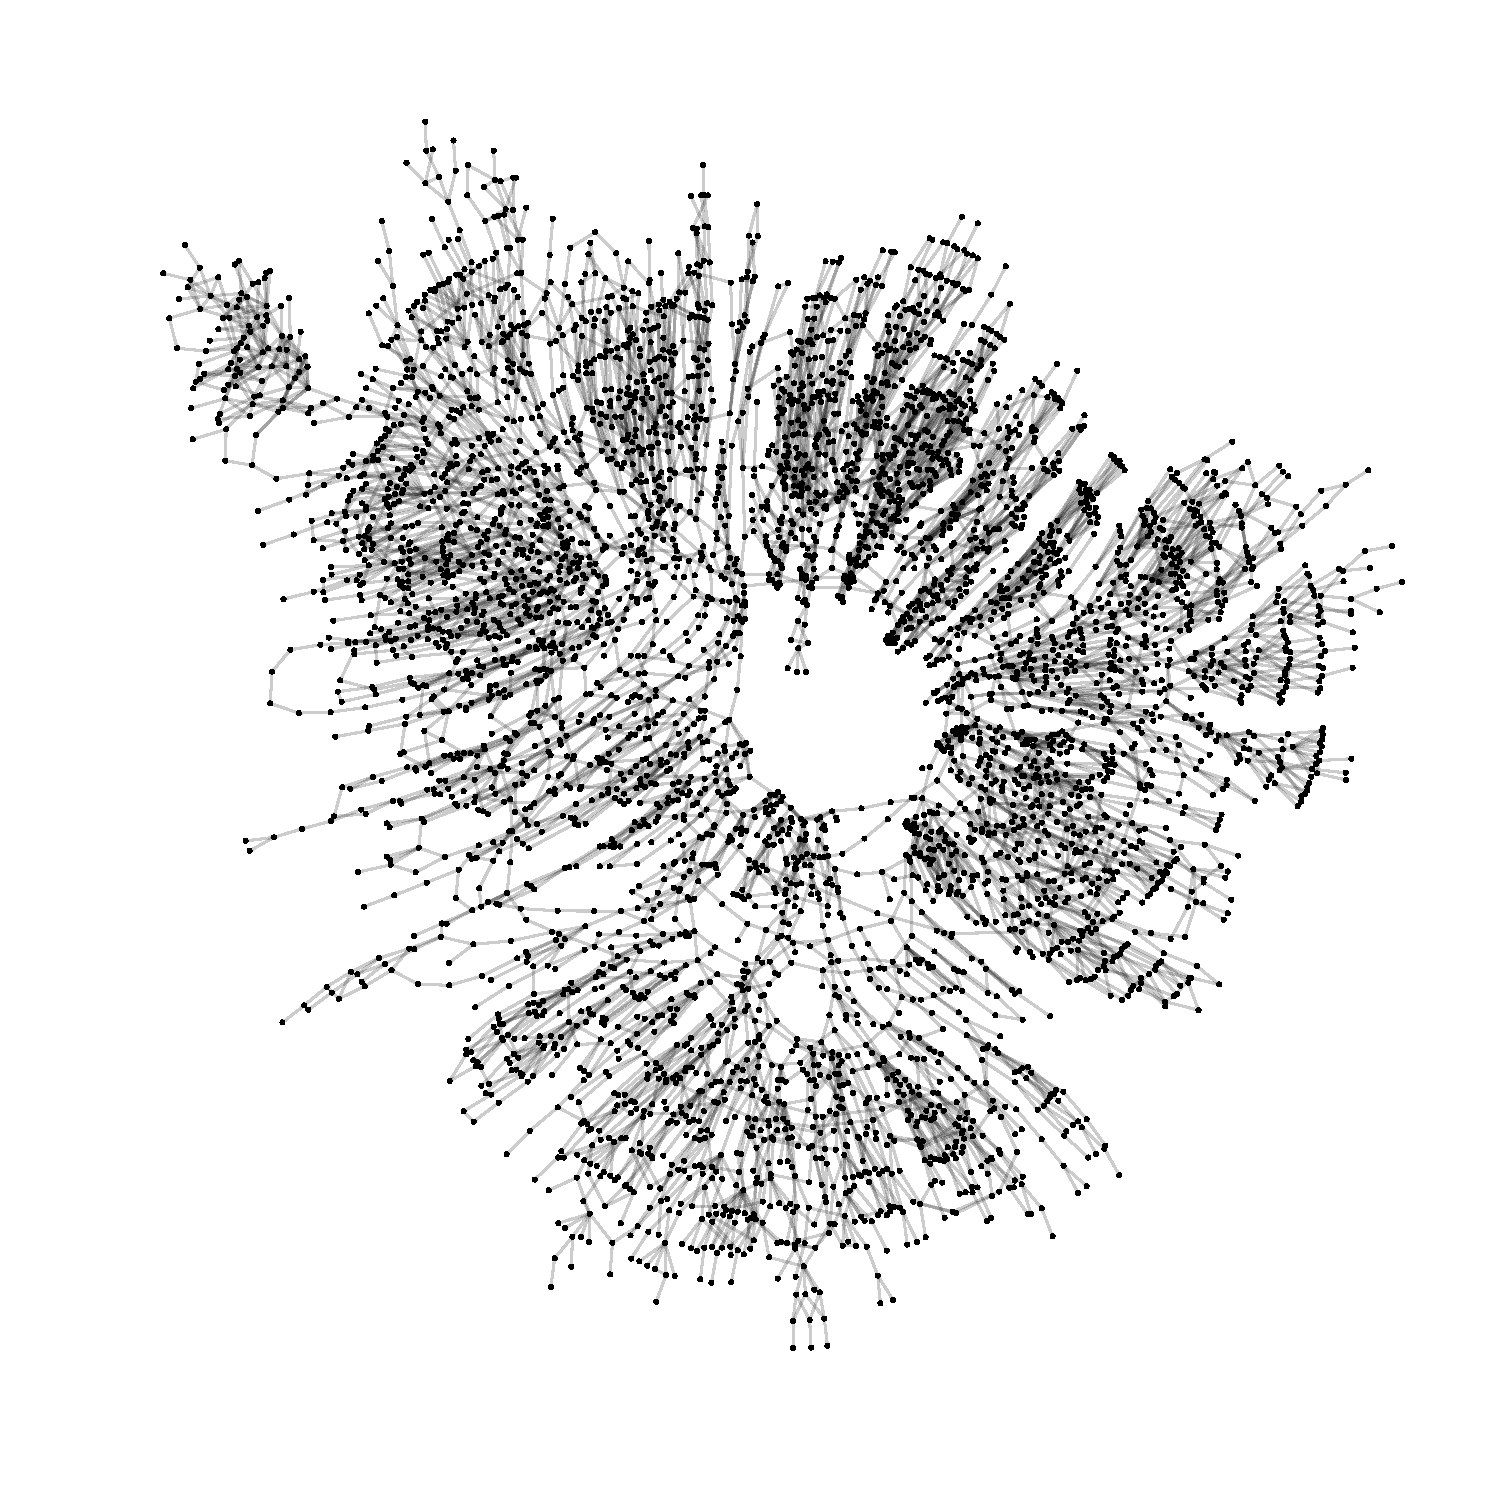
\includegraphics[width=\textwidth]{network-US-power-grid.pdf}
	\caption{Power grid network of the Western States of USA. Nodes represent electrical stations (generator, transformator, substation) and edges represent power supply lines. Data retrieved from the Konect database \cite{kunegis2013konect} (Konect code \code{UG}).}
	\label{Figure: Network of western US powergrid}
\end{figure}

\begin{figure}
	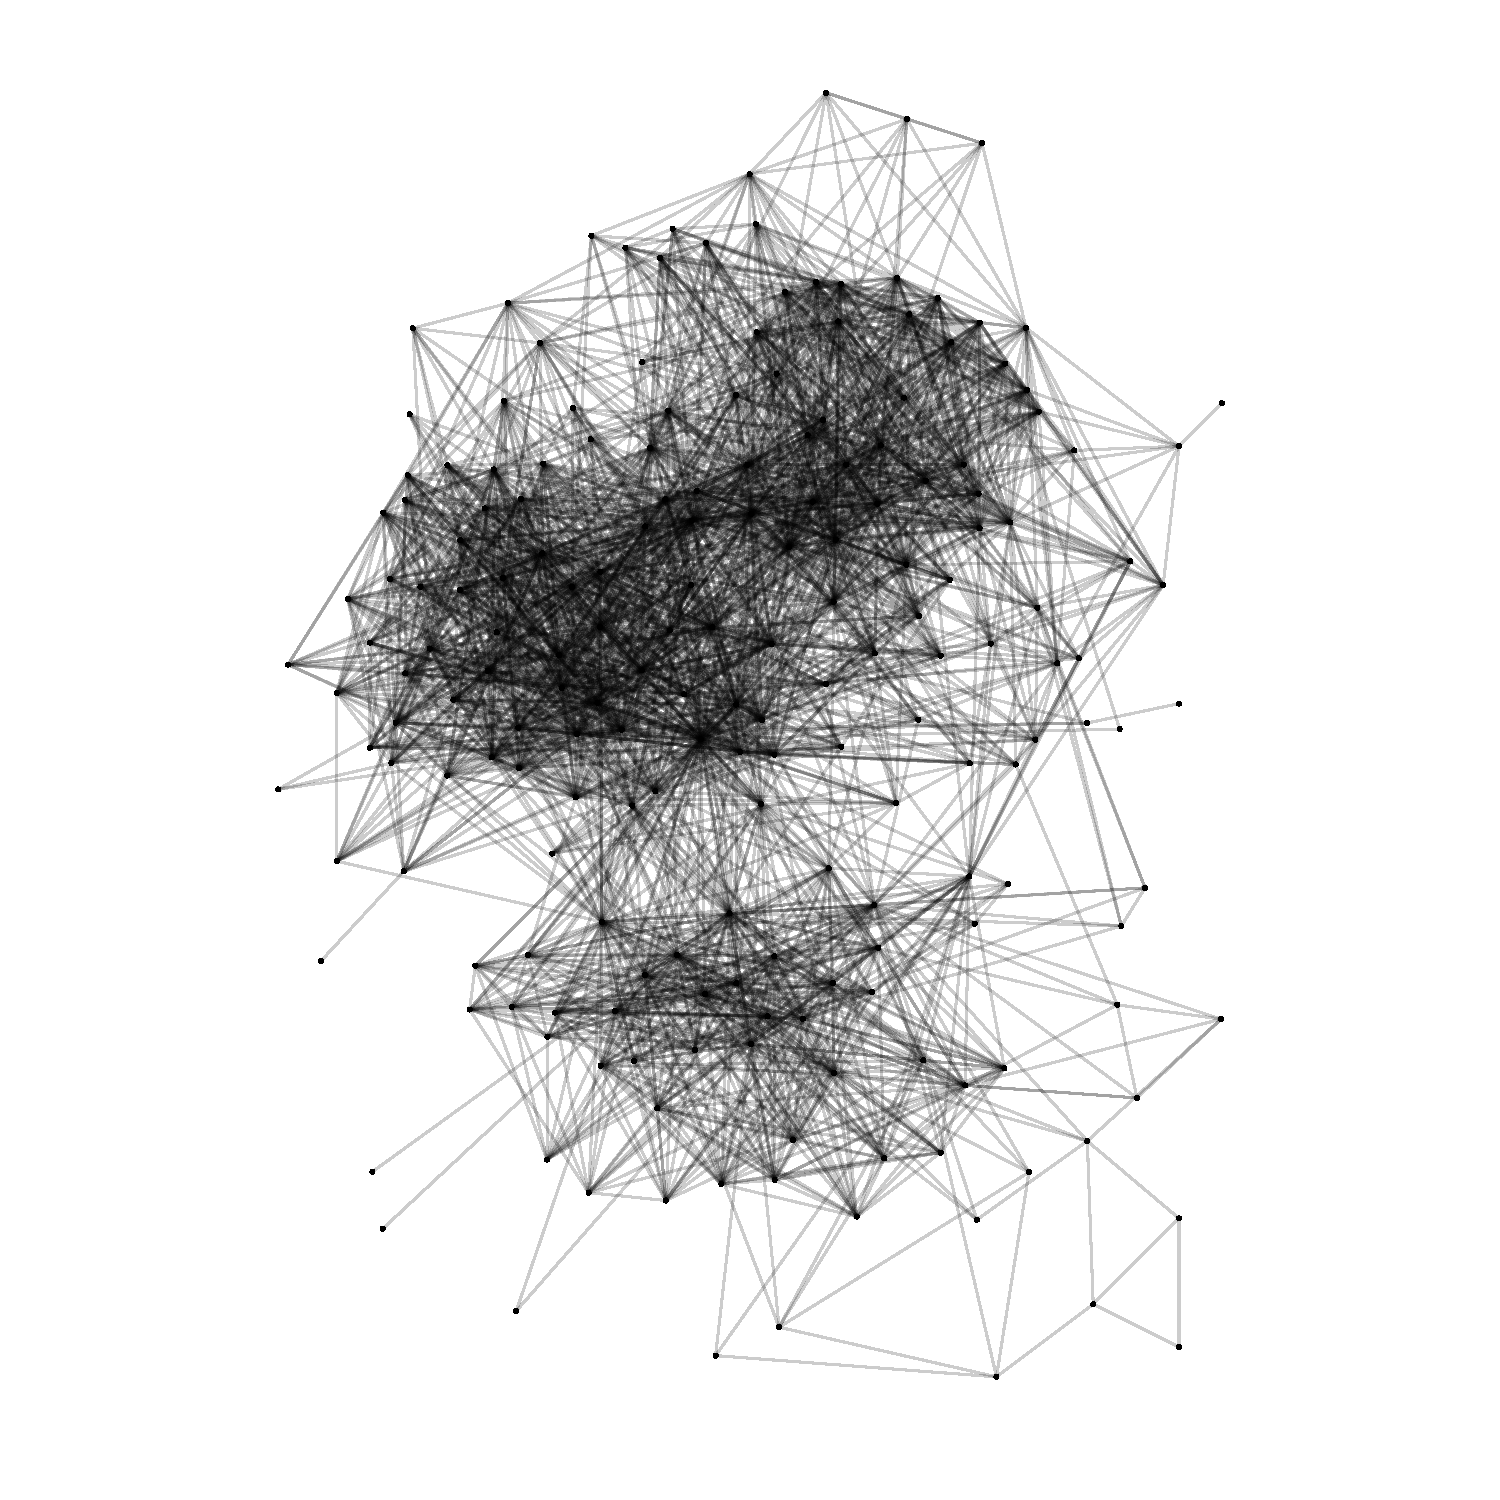
\includegraphics[width=\textwidth]{network-arenas-jazz.pdf}
	\caption{Collaboration network of jazz musicians as of 2003. Nodes represent musicians and edges represent the fact that the two musicians had played in the same band. Data retrieved from the Konect database \cite{kunegis2013konect} (Konect code \code{JZ}).}
	\label{Figure: Network of jazz musicians collaborations}
\end{figure}

\begin{figure}
	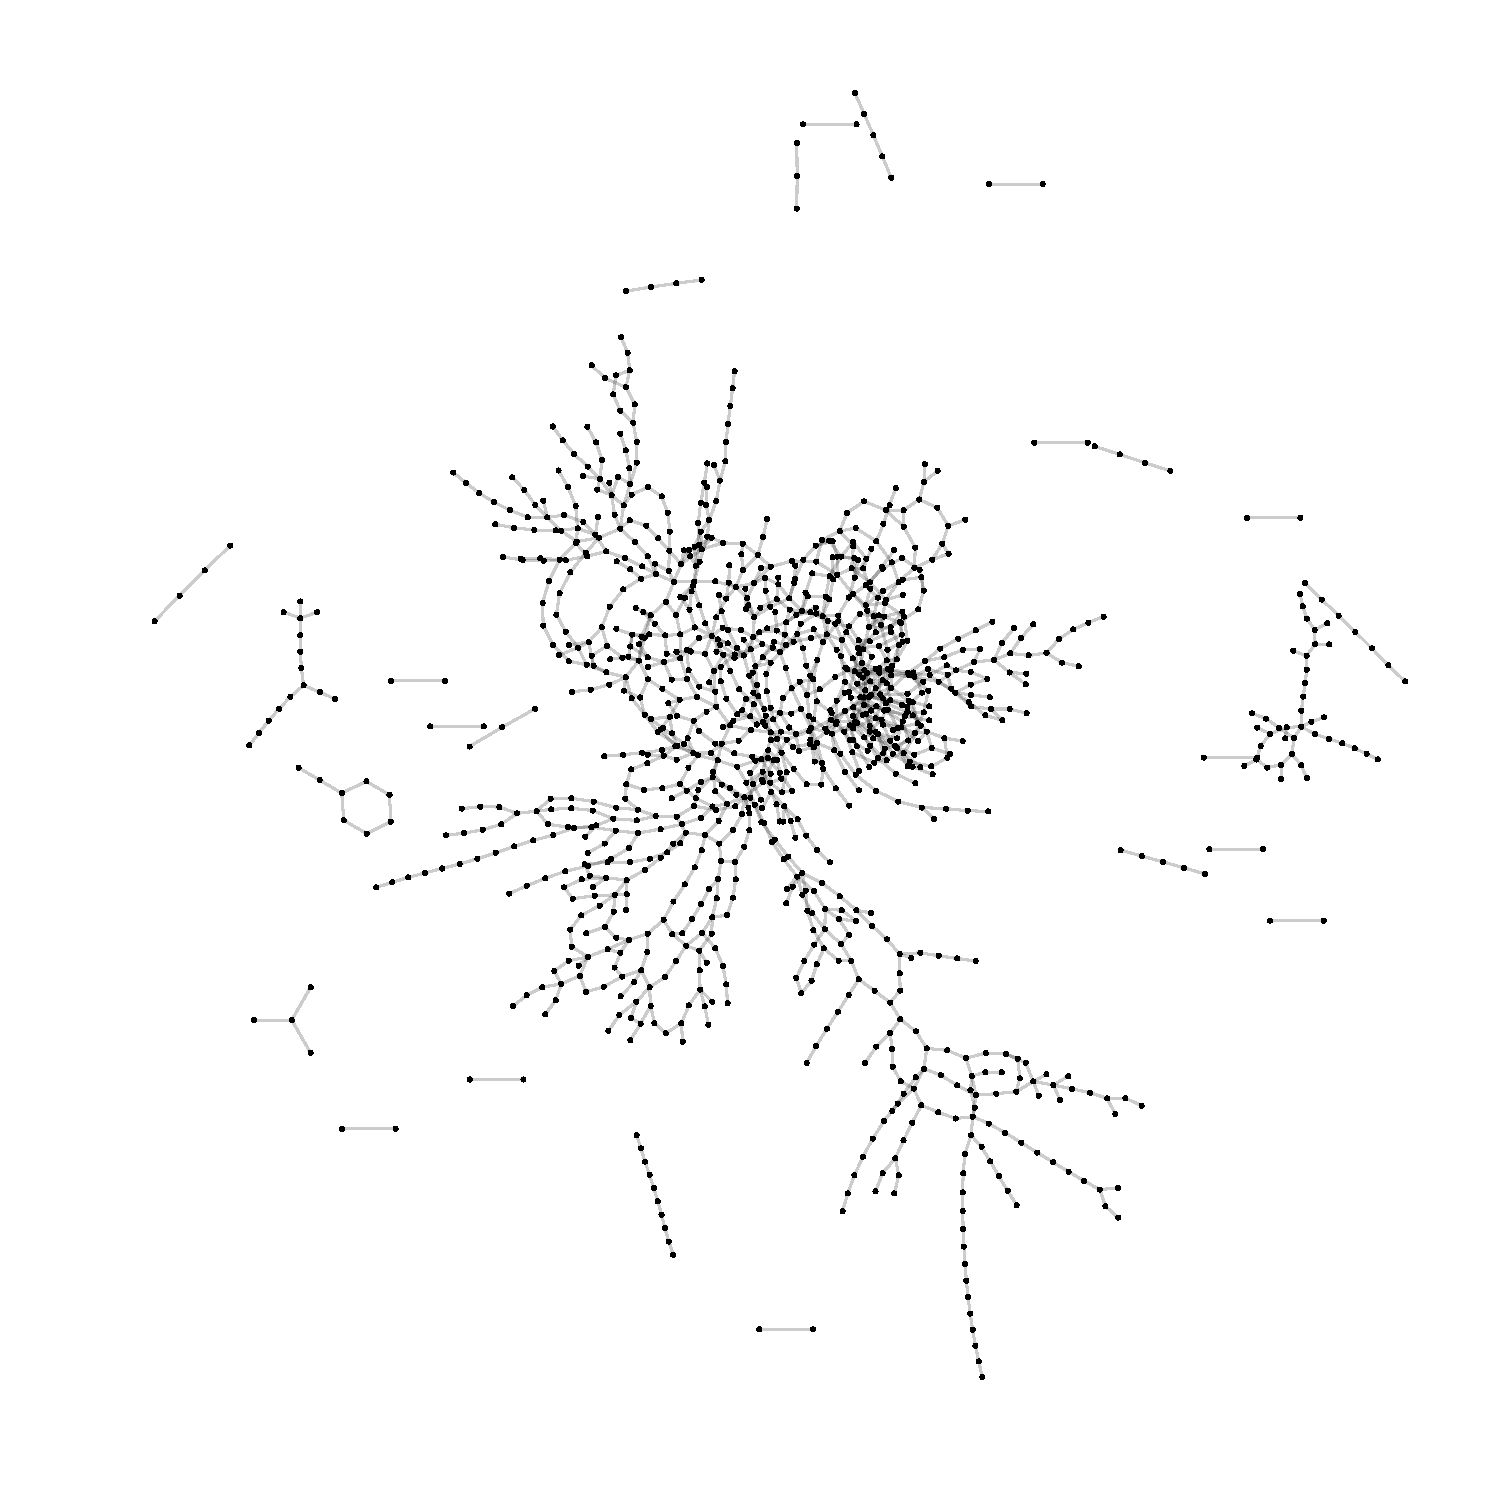
\includegraphics[width=\textwidth]{network-subelj_euroroad.pdf}
	\caption{International E-road network, a network of road situated mainly in Europe. Nodes represent cities and edges represent E-roads connecting them. Data retrieved from the Konect database \cite{kunegis2013konect} (Konect code \code{ET}).}
	\label{Figure: Network euroroad}
\end{figure}

\begin{figure}
	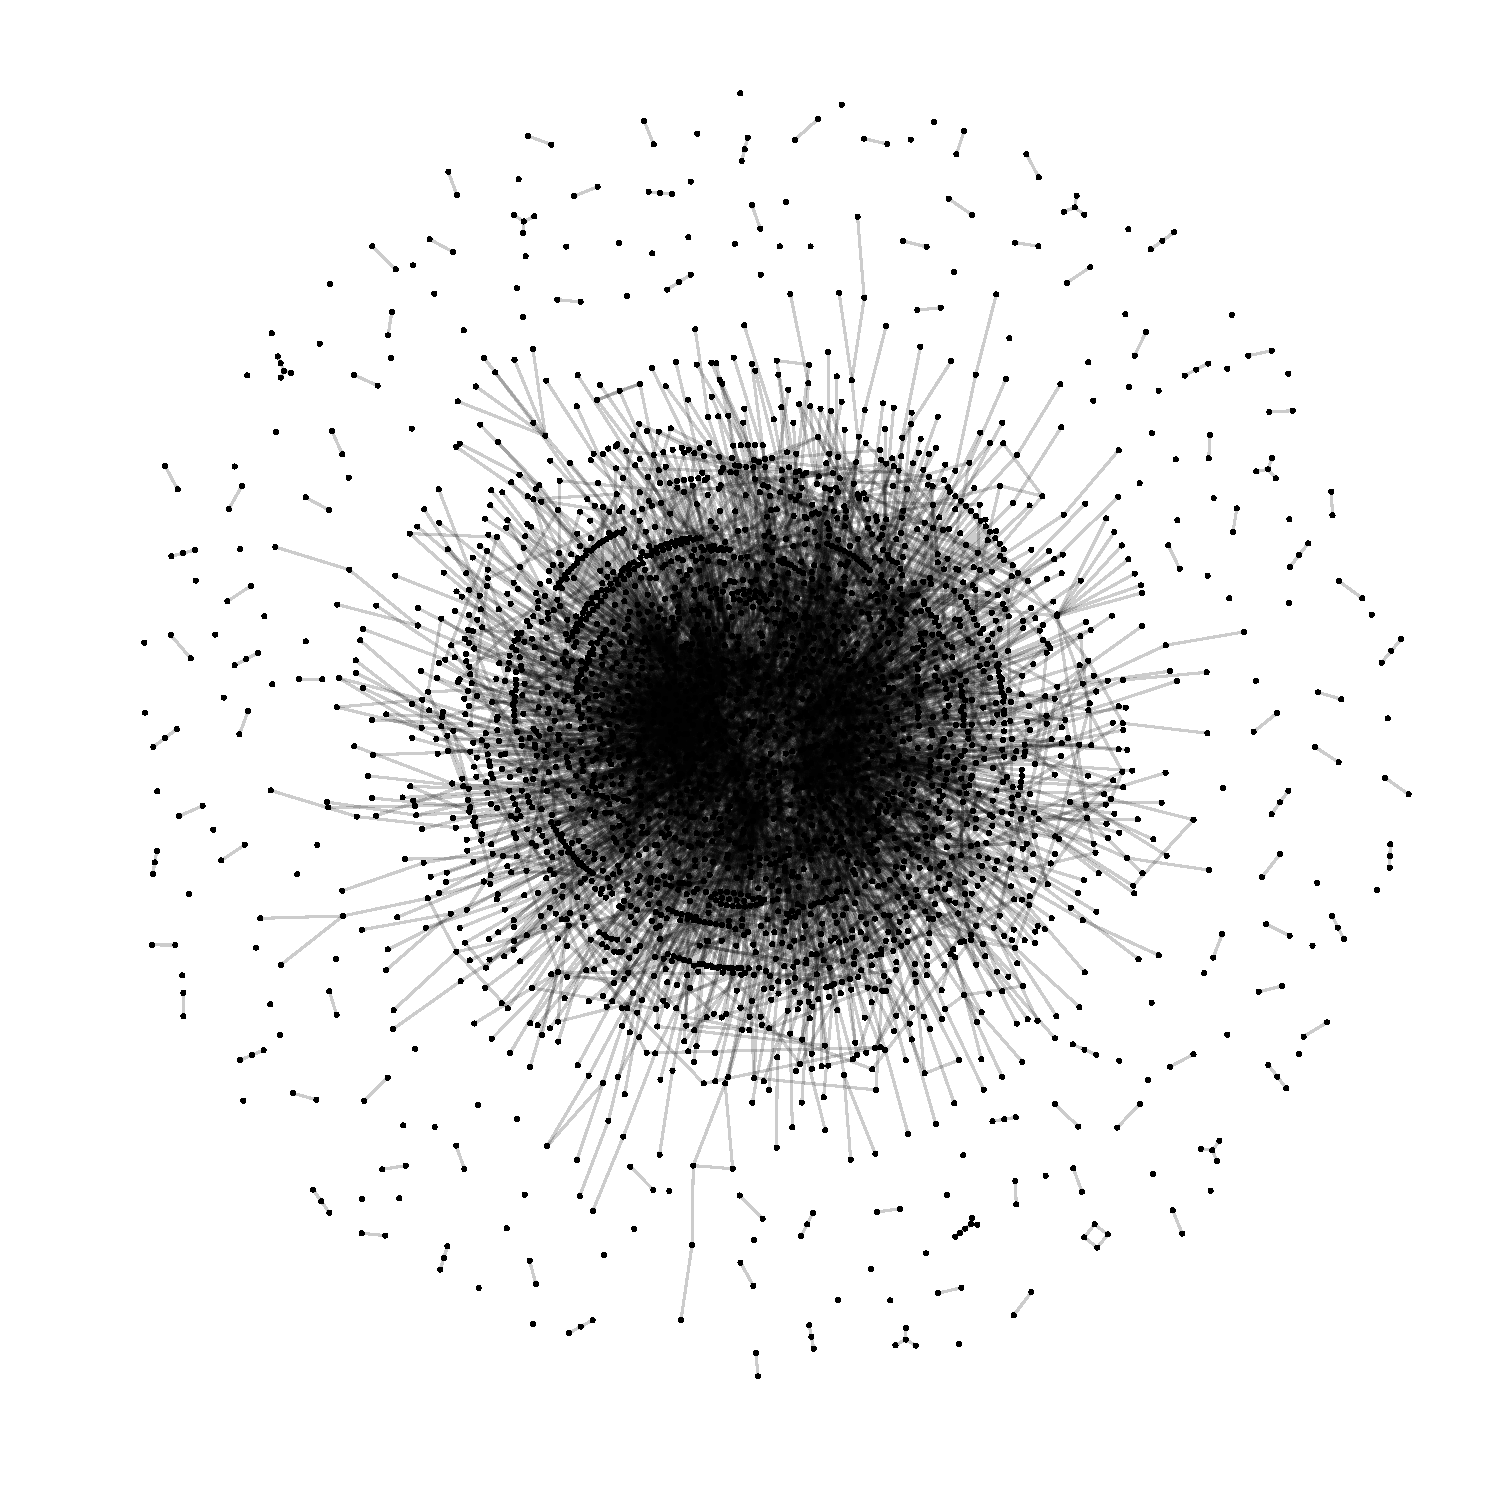
\includegraphics[width=\textwidth]{network-maayan-vidal.pdf}
	\caption{Network of protein-protein interaction in humans. Nodes represnt proteins and edges a binary interaction. Data retrieved from the Konect database \cite{kunegis2013konect} (Konect code \code{MV}).}
	\label{Figure: Network of human proteins}
\end{figure}


Mathematically, networks are represented as \newconcept{graphs}. A graph is an object composed of a set $V$ of \newconcept{vertices} (also referred to as nodes) and a set of \newconcept{edges} $E$. An edge is characterized by the fact that it connects two vertices together, which in mathematical terms translate to the fact that an edge can be written as a pair of vertices or equivalently $E \subset \set{(v_1, v_2) | v_1, v_2 \in V }$. Many extensions of this model exist, for example edges may have a direction (\newconcept{directed graph}), implying that $(v_1, v_2) \neq (v_2, v_1)$, or edges can carry a value (\newconcept{weighted graph}).

In this first chapter we focus on the standard unweighted and undirected networks, even restricting our theoretical analysis to the case of infinitely large networks as it allows for several convenient simplifications while still capturing important feature networks. In Chapter \ref{Section: Multiplex networks} we study an extension of this network category, multiplex networks, which consists in allowing distinct type of edges between the vertices.

\section{Configuration model}
\label{Section: Configuration model}

Since we are interested in fundamental properties of networks, we need to abstract from the specificity of one network. To do so, we consider that networks are fully determined by their \newconcept{degree distribution} $\set{p_k}$ where $p_k$ is the probability for a node chosen randomly and uniformly to have degree $k$. Since knowing how a network can be constructed is useful both conceptually and to perform computation on properties of the network, we now present an algorithm called \newconcept{configuration model} \cite{newman2010networks} that sample uniformly the space of all network with a given degree distribution.

Consider a network with $n$ vertices with a given degree distribution $\set{p_k}$. If we cut every edges in two, every vertex keep a number of \newconcept{stubs} (half-edges) equal to its degree. The resulting set of vertices and stubs is independent of the network structure, but common for all networks with the same degree distribution. The idea of this algorithm is thus to start from this state, a set of nodes with stub degree distribution $\set{p_k}$. Then each stub is bond to another chosen uniformly amongst other stubs to form all edges of the network. By construction, the produced network has degree distribution $\set{p_k}$.

The fact that stubs are paired uniformly and independently is important in that it implies that the vertex reached by following a random edge does not dependant, in probability, on the vertex at the other end of the edge.

\todo[inline]{Think about that and the need for that for GCC calculation}

\section{Self-edges and multi-edges}

\begin{figure}
	{
\newcommand{\configurationmodelexamplepoints}
{
	\node[node] (A) at (0.2, 0) {} ;
	\node[node] (B) at (1, 1.5) {} ;
	\node[node] (C) at (-0.7, 1.2) {} ;
	\node[node] (D) at (-0.5, -0,1) {} ;
	\node[node] (E) at (1.7, -0.6) {} ;
}

\newcommand{\legendpos}{(0.2, -1.5)}


\begin{tikzpicture}
	\configurationmodelexamplepoints
	
	\draw (A) -- ++(0.4, 0.3) ;
	\draw (A) -- ++(-0.5, 0) ;
	\draw (A) -- ++(-0.3, 0.4) ;
	
	\draw (B) -- ++(0.4, -0.3) ;
	\draw (B) -- ++(-0.4, -0.3) ;
	
	\draw (C) -- ++(-0.3, -0.4) ;
	\draw (C) -- ++(0.5, 0) ;
	
	\draw (D) -- ++(-0.3, 0.4) ;
	
	\draw (E) -- ++(-0.4, -0.3) ;
	\draw (E) -- ++(0, 0.5) ;
	
	\node (leg) at \legendpos {(A) Nodes and theirs stubs} ;
\end{tikzpicture}
\hspace{1cm}
\begin{tikzpicture}
	\configurationmodelexamplepoints
	
	\draw (A) -- (B) ;
	\draw (A) -- (C) ;
	\draw (A) -- (E) ;
	\draw (B) -- (E) ;
	\draw (C) -- (D) ;
	
	\node (leg) at \legendpos {(B) Stubs are randomly connected} ;
\end{tikzpicture}
}
	\caption{Schematic representation of the configuration model.}
	\label{Figure: Configuration model}
\end{figure}

Using the insight given by the algorithm, we can compute the probability that a node is connected to itself, thus making a so-called \newconcept{self-edge}. In a network with $m$ edges, there are $2 m$ stubs. The probability $p_{ii}$ that a stub of vertex $i$ connect to another stub of the same vertex is thus
\begin{align}
	p_{ii} = m \frac{ \begin{pmatrix} k_i \\ 2 \end{pmatrix} }{ \begin{pmatrix} 2m \\ 2 \end{pmatrix} } = \frac{k_i (k_i - 1)}{2 (2m - 1)},
\end{align}
where $k_i$ is the degree of vertex $i$. In the limit of large $n$, the number of vertices with degree $k$ is equal to $n p_k$ and as a consequence the total number $m$ of edges is equal to
\begin{align}
	m = \frac{1}{2} \sum_{k = 0}^\infty n k p_k = \frac{n}{2} \expected{\deg{v}},
\end{align}
with $\expected{\dots}$ denoting the expectation value. The average number of self-edges is therefore asymptotically constant as $n$ becomes large, so the fraction of vertices having self edges goes to zeros as $n$ grows and we can safely consider the generated network has no self-edges at all.

Similarly, we find that the probability $p_{ij}$ that two vertices $i$ and $j$ are connected is equal to
\begin{align}
	p_{ij} = m \frac{k_i k_j}{ \begin{pmatrix} 2m - 2 \\ 2 \end{pmatrix} } = \frac{k_i k_j}{2 m -1}.
\end{align}
The probability to have two or more edges between the vertices $i$ and $j$ is equal to the probability that $i$ and $j$ are connected and that they remain so after we remove one edge between them. The probability for them to be connected with one edge less is the same as $p_{ij}$ but with one edge less in total and one stub less at both $i$ and $j$, giving
\begin{align}
	\frac{(k_i - 1)(k_j - 1)}{2 m - 3}.
\end{align}
In consequence we find the probability to have at least two edges between $i$ and $j$ to be
\begin{align}
	p_{ij} \frac{(k_i - 1)(k_j - 1)}{2 m - 3},
\end{align}
giving the average number of multi-edges
\begin{align}
	\frac{\sum_{ij} k_i k_j (k_j - 1) (k_i - 1)}{2 (2 m - 1)(2 m - 3)}  &\approx \frac{1}{8 m^2} \sum_i k_i(k_i - 1) \sum_j k_j(k_j - 1) \\
	&= \frac{1}{2}\left[ \frac{\expected{(\deg{v})^2} - \expected{\deg{v}}}{\expected{\deg{v}}} \right]^2.
\end{align}
The approximation arise as in the limit of large $n$ we have $2 m - 3 \approx 2 m - 3 \approx 2 m$ as $m$ scale proportionally to $n$. As in the case of self-edges, the number of multi-edges is asymptotically constant and we can therefore consider that the generated networks has no multi-edges.

Since $\set{p_k}$ is a probability distribution, it is independent of the number of nodes $n$ of the network. Therefore for any degree distribution, we can consider the limit for large $n$, which we do as it allows several mathematical simplifications of the problem as outlined below. For sufficiently large networks, the difference between the large $n$ limit and the actual network is small and can thus safely be neglected.

A network having this two properties, absence of self-edges and of multi-edges, is said to be a \newconcept{simple graph}. Since for $n$ large enough all networks in the context of the configuration model have approximately these two properties, we always consider that the networks are simple graphs in the remaining of this thesis.

\section{Uniformity of network space sampling}

In the previous section we demonstrated that the configuration model asymptotically produces simple graphs in the limit of large $n$. This is necessary to prove the claims we make in Section \ref{Section: Configuration model} that the configuration uniformly sample the space of networks with a given degree distribution. To prove that claim is equivalent to prove that each different network appears with the same probability.

\todo[inline]{The following calculation is not correct, nodes with the same degree are indistinguishable as well. Correct and note the disagreement with Newman}

A \emph{matching} of the stubs is a possible way to bond $2 m$ distinguishable stubs. By construction the pair of stubs that are bound are chosen uniformly and thus each matching appears with the same probability than any other. However, in practice the stubs of a single vertex are not distinguishable and several matching leads to the same network. Therefore there is $k!$ way of arranging the stubs of a vertex of degree $k$, resulting in a total of
\begin{align}
	\prod_{i = 1}^n k_i!
\end{align}
matchings corresponding to the same network, where $k_i$ is the degree of vertex $i$. This quantity only depends on the degree distribution, thus all networks with the same degree distribution have the same number of different matchings. Since each matching appears with the same probability, we can conclude that each network with a given degree distribution appears with the same probability in the configuration model.

In a sense the configuration model is therefore optimal for the point of view we adopt in this thesis. Indeed we consider a network fully determined by its degree distribution and all network with a common degree distribution are equal with regard to the configuration model as it sample them uniformly. We could in fact present the configuration model as a consequence of the requirement that we want a sampling method introducing no unnecessary constrain on the produced networks. See Section 15.2 of \cite{newman2010networks} or \missingref[maximum entropy paper] for discussions of that point of view.

\section{Excess degree distribution}

As we will see below, while we consider that a network is fully determined by its degree distribution, considering vertices reached by following an edge gives valuable insights on the network structure. We call such vertex a \newconcept{first neighbor} vertex and we denote $P_1(\dots)$ the probability associated with a first neighbor, while we denote $P_0(\dots)$ the probability associated with uniformly chosen vertices\footnote{In principle $P_j(\dots)$ could be defined, corresponding to the probability associated with vertices reached after following $j$ edges.}. We can define the \newconcept{excess degree distribution} $\set{q_k}$ as
\begin{align}
	q_k = P_1(\deg{v} = k + 1), \qquad \forall k \in \mathbb{N}.
\end{align}
The probability $q_k$ correspond to a first neighbor having degree $k + 1$, or equivalently to the probability to have $k$ edges other than the on used to reach the node in the first place, hence the name excess degree distribution.

The excess degree distribution can be computed explicitly by noting that a stub has the same probability to be connected to any if the other $2 m - 1$ stubs, thus the probability that this stub is connected to a given node of degree $k$ is $k/(2 m - 1)$. Multiplying by the total number of node of degree $k$, $n p_k$ in the large $n$ limit,gives the probability that a given node is attached to a node of degree $k$ as
\begin{align}
	\frac{k}{2 m -1} n p_k = \frac{k p_k}{\expected{\deg{v}}}.
\end{align}
Now $q_k$ is the probability that a first neighbor has degree $k + 1$, so we can conclude
\begin{align}
	q_k = \frac{(k + 1) p_{k+1}}{\expected{\deg{v}}}. \label{qk as function of pk}
\end{align}

\section{Generating functions}
\label{Section: Generating functions}

A powerful way of representing a degree distribution (or any discrete probability law) is the \newconcept{generating function} of the distribution. For a degree distribution $\set{p_k}$ it is defined as the function
\begin{align}
	g_0(z) = \sum_{k=0}^\infty p_k z^k. \label{Definition of g0}
\end{align}

Observe that the derivative with respect to $z$ of $g_0(z)$ is
\begin{align}
	g'_0(z) = \sum_{k=0}^\infty p_k k z^{k-1}. \label{Derivative of g0}
\end{align}
Comparing with definition of the expectation value we find
\begin{align}
	\expected{\deg{v}} = \sum_{k=0}^\infty p_k k = g'_0(1). \label{Expectation value as g'0(1)}
\end{align}
Therefore, the generating function is sufficient to know the expectation value of a distribution. This result can be generalized: if we look at the second derivative of the generating function, by differentiating eq. \eqref{Derivative of g0}, we find
\begin{align}
	g''_0(1) &= \sum_{k=0}^\infty p_k k (k - 1) = \sum_{k=0}^\infty p_k k^2 - \sum_{k=0}^\infty p_k k \\
		&= \expected{(\deg{v})^2} - \expected{\deg{v}}.
\end{align}
Thus we can write
\begin{align}
	\expected{(\deg{v})^2} &= g''_0(1) + g'_0(1) = \frac{\partial}{\partial z}\left(z g'_0(z)\right)\evaluatedat{z = 1},  \label{Second moment as derivatives of g0}
\end{align}
which means that the second moment is fully determined by the generating as well. In fact such formula exists for all moments, but we do not present it here as we only need the first two moments. The second moment is used to compute the variance of the degree distribution as follow
\begin{align}
	\var{\deg{v}} &= \expected{(\deg{v})^2} - \left(\expected{\deg{v}}\right)^2 \\
		&= \frac{\partial}{\partial z}\left(z g'_0(z)\right)\evaluatedat{z = 1} - \left(g'_0(1)\right)^2. \label{Variance as derivatives of g0}
\end{align}

All these properties do not depend on the degree distribution $p_k$ to which the generating function is associated and apply to any discrete probability distribution. One other important distribution for network is the excess degree distribution $\set{q_k}$, we define its generating function $g_1$ as
\begin{align}
	g_1(z) = \sum_{k=0}^\infty q_k z^k. \label{Definition of g1}
\end{align}

Inserting eq. \eqref{qk as function of pk} in this definition, we get
\begin{align}
	g_1(z) = \frac{1}{\expected{\deg{v}}} \sum_{k=0}^\infty (k + 1) p_{k + 1} z^k = \frac{g'_0(z)}{g'_0(1)}, \label{g1 as a function of g0}
\end{align}
where we used eq. \eqref{Derivative of g0 for scale free networks} and eq, \eqref{Expectation value as g'0(1)} for the last equality.

\section{Erdos-Renyi networks}

In this thesis we focus on three types of theoretical networks, beside some real examples: Erdos-Renyi networks, scale-free networks and geometric networks.

An Erdos-Renyi networks is characterized by the fact that it can be grown as follow: for each pair of nodes $i$ and $j$, add an edge with probability $p$. To find the degree distribution in such network, first notice that the expected degree, usually denoted $c$ for Erdos-Renyi network, is equal to the number of other vertices multiplied by the probability to be connected to each of them, i.e.
\begin{align}
	c = \expected{\deg{v}} = (n - 1) p.
\end{align}
We generally use $c$ as the parameter defining an Erdos-Renyi network, rather than $p$, since it makes more to keep $c$ constant when $n$ becomes large, rather than $p$. 

The probability for a node to have degree $k$ is
\begin{align}
	p_k = \nchoosek{n-1}{k} p^k (1 - p)^{n - 1 - k}, \qquad \forall k \in \mathbb{N}. \label{Poisson degree distribution}
\end{align}
We recognize a binomial degree distribution for $n-1$ trials with success probability $p$. In the limit of large $n$ we can approximate such distribution by a Poisson distribution with parameter $c = (n - 1) p$
\begin{align}
	p_k \approx \frac{c^k}{k!} e^{-c}.  \label{pk for Erdos-Renyi}
\end{align}
The parameter $c$ is the expected degree in the network, it is proportional to $n - 1$ rather than $n$ because we only tries to bind each vertex with each other, and not with itself, making a total of $n-1$ trials.

Inserting the degree distribution in the definition of the generating function \eqref{Definition of g0}, we recognize Taylor series representing the exponential function and thus we get
\begin{align}
	g_0(z) = e^{-c} \sum_{k = 0}^\infty \frac{z^k c^k}{k!} = e^{-c} e^{c z} = e^{c(z - 1)}. \label{g0 for ER networks}
\end{align}
Taking the derivative and inserting in eq. \eqref{Definition of g1} yields the generating function for the excess degree distribution
\begin{align} 
	g_1(z) = e^{c(z - 1)},
\end{align}
which appears to be equal to $g_0(z)$.

\section{Geometric networks}

Geometric networks have a geometric degree distribution
\todo[inline]{Ask Guiyuan which version to use and if there is a some motivation in using this geom. dist.}

\section{Scale-free networks}

The degree distribution of a so-called scale-free network follows a power law with exponent $\alpha$
\begin{align}
	p_k = \frac{k^{-\alpha}}{\zeta(\alpha)}, \qquad \forall k \in \mathbb{N}^*, \label{Power law degree distribution}
\end{align}
where $\zeta(\alpha)$ is the Riemann zeta function and $p_0 = 0$. This kind of networks is interesting as many real networks exhibits power law tail in their degree distribution \todo{Add examples}. However, power law distribution are mathematically more complicated than the two previous examples as their generating function can not be represented in term of elementary function. The best we can do is introducing the \newconcept{polylogarithm} $\polylog{\alpha}{z}$
\begin{align}
	\polylog{\alpha}{z} = \sum_{k=1}^\infty k^{-\alpha} z^k. \label{Definition of polylogarithm}
\end{align}
The polylogarithm is a generalization of the Riemann zeta function, as can be seen by the fact that for $z = 1$ we have
\begin{align}
	\polylog{\alpha}{1} = \sum_{k=1}^\infty k^{-\alpha} = \zeta(\alpha) \label{Polylogarithm of 1}.
\end{align}
\todo[inline]{Credit the guy the polylog code comes from. Maybe say a bit more about polylog/reimplement polylog using intergation}

With that notation, the generating function $g_0(z)$ for scale-free networs can be written
\begin{align}
	g_0(z) = \sum_{k=1}^\infty \frac{k^{-\alpha}}{\zeta(\alpha)} z^k = \frac{\polylog{\alpha}{z}}{\zeta(\alpha)}. \label{Generating function for scale free networks}
\end{align}

While no simple expression exist for the polylogarithm, its formal definition \eqref{Definition of polylogarithm} is sufficient to compute its derivative
\begin{align}
	\frac{\partial}{\partial z} \polylog{\alpha}{z} = \sum_{k = 1}^\infty k^{-\alpha + 1} z^{k-1} = \frac{1}{z} \polylog{\alpha - 1}{z}. \label{Derivative of the polylogarithm}
\end{align}
We therefore find
\begin{align}
	g'_0(z) = \frac{\polylog{\alpha - 1}{z}}{z \zeta(\alpha)}  \label{Derivative of g0 for scale free networks}
\end{align}
that we can insert in eq. \eqref{g1 as a function of g0} to get
\begin{align}
	g_1(z) =  \frac{\polylog{\alpha - 1}{z}}{z \zeta(\alpha - 1)}.
\end{align}
We used eq. \eqref{Polylogarithm of 1} to perform the simplification $g'_0(1) = \zeta(\alpha - 1)/\zeta(\alpha)$. Thanks to eq. \eqref{Expectation value as g'0(1)}, we know that $g'_0(1) = \expected{\deg{v}}$. Thus we have
\begin{align}
	\expected{\deg{v}} = \frac{\zeta(\alpha - 1)}{\zeta(\alpha)}. \label{Mean degree in scale free network}
\end{align}

Since we are not considering the analytic continuation of the zeta function, but only its real sum description given in eq. \eqref{Polylogarithm of 1}, $\zeta(\alpha)$ diverges for $\alpha < 1$. We can therefore distinguish three cases. First for $\alpha \leq 2$, eq. \eqref{Mean degree in scale free network} diverges and the mean degree always goes to infinity as the network grows. The name scale free comes from that fact, as there is no \emph{typical scale} for the degrees and greater degrees can always happen with probability too high to be ignored.

In the case $2 < \alpha \leq 3$, the mean degree is finite, but its second moment is not. It can be seen by calculating explicitly using using eq. \eqref{Second moment as derivatives of g0},
\begin{align}
	\expected{(\deg{v})^2} &= \frac{\partial}{\partial z}\left(z g'_0(z)\right)\evaluatedat{z = 1} = \frac{\partial}{\partial z}\left(\frac{\polylog{\alpha - 1}{z}}{\zeta(\alpha)} \right)\evaluatedat{z = 1} \\
		&= \frac{\polylog{\alpha - 2}{1}}{\zeta(\alpha)} = \frac{\zeta(\alpha - 2)}{\zeta(\alpha)}.
\end{align} 
The divergence of the second moment come from the fact that the factor $\zeta(\alpha - 2)$ diverges for $\alpha \leq 3$. In consequence, the variance of the degree distribution diverges, which means the degree are very widely distributed.

A nicer interpretation arises from a consequence of eq. \eqref{g1 as a function of g0}, namely
\begin{align}
	g'_1(1) = \frac{g''_0(z)}{g'_0(z)}.
\end{align}
A similar calculation as for the second moment shows that for $\alpha \leq 3$, this diverges too. Hence, for $2 < \alpha \leq 3$ the degree distribution is not strictly speaking scale free, but the excess degree distribution is.

Finally for $\alpha > 3$, the two first moment are finite and only higher moments diverge, which does not implies any peculiar behavior.

\section{Giant connected component}
\label{Section: Giant connected component}

\subsection{Size of the GCC}

An interesting property of a network is the presence and size of \newconcept{connected component}. A set of nodes is said to be connected if there is a path formed of successive edges from any of its node to any other. All networks can be divided in connected components such that all nodes are element of exactly one component, as is exemplified in fig. \ref{Figure: Connected components}. The connectedness of network is crucial in many real world realisations of networks. In particular any logistic network, such as power grid networks, rail road network or the internet network, is functional only if it is able to transfer goods or services (electricity, passengers or informations) from any node to any other.

\begin{figure}
	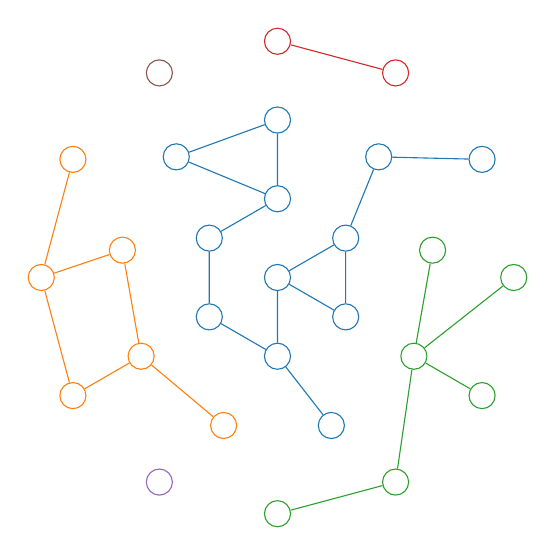
\begin{tikzpicture}
	\node (A') at (0, 0) {} ;
	
	\foreach \n in {1, 2, ..., 6}
	{
		\node (B\n') at ({sin(\n*360/6)}, {cos(\n*360/6)}) {} ;
	}
	
	
	\foreach \n in {1, 2, ..., 9}
	{
		\node (C\n') at ({2*sin(\n*360/9)}, {2*cos(\n*360/9)}) {} ;
	}
	
	
	\foreach \n in {1, 2, ..., 12}
	{
		\node (D\n') at ({3*sin(\n*360/12)}, {3*cos(\n*360/12)}) {} ;
	}
	
	\newcommand{\compcolor}{C0}
	\foreach \cooname in {A, B1, B2, B3, B4, B5, B6, C1, C4, C8, C9, D2}
	{
		\node[node, \compcolor] (\cooname) at (\cooname') {} ;
	}
	\draw[\compcolor] (A) -- (B1) -- (B2) -- (A) ;
	\draw[\compcolor] (A) -- (B3) -- (C4) ;
	\draw[\compcolor] (B1) -- (C1) -- (D2) ;
	\draw[\compcolor] (B3) -- (B4) -- (B5) -- (B6) -- (C9) -- (C8) -- (B6) ;
	
	
	\renewcommand{\compcolor}{C1}
	\foreach \cooname in {C5, C6, C7, D8, D9, D10}
	{
		\node[node, \compcolor] (\cooname) at (\cooname') {} ;
	}
	\draw[\compcolor] (D10) -- (D9) -- (D8) -- (C6) -- (C7) -- (D9) ;
	\draw[\compcolor] (C6) -- (C5) ;
	
	
	\renewcommand{\compcolor}{C2}
	\foreach \cooname in {C2, C3, D3, D4, D5, D6}
	{
		\node[node, \compcolor] (\cooname) at (\cooname') {} ;
	}
	\draw[\compcolor] (C2) -- (C3) -- (D5) -- (D6) ;
	\draw[\compcolor] (D3) -- (C3) -- (D4) ;
	
	
	\renewcommand{\compcolor}{C3}
	\foreach \cooname in {D1, D12}
	{
		\node[node, \compcolor] (\cooname) at (\cooname') {} ;
	}
	\draw[\compcolor] (D12) -- (D1) ;
	
	
	\node[node, C4] (D7) at (D7') {} ;
	\node[node, C5] (D11) at (D11') {} ;
\end{tikzpicture}
	\caption{Scheme of a graph with six connected components, each drawn with a different color.}
	\label{Figure: Connected components}
\end{figure}

Insight on the property of networks can be found by studying the case where the fraction of the network forming its biggest component does not vanish in the large $n$ limit. This component is called the \newconcept{giant connected component} (GCC). The first question to answer about it is: what will be the size of the giant connected component ?

To determine this consider a connected component $C$ of the network. We define $u$ the probability that a node reached by following an edge is not part of $C$. We can therefore write the probability $S$ that a randomly chosen vertex is part of $C$ as
\begin{align}
	S 	&= 1 - P_0(w \notin C\; \forall w \in N(v))\\
		&= 1 - \sum_{k=0}^\infty P_0(w \notin C\; \forall w \in N(v)|\deg{v} = k) P_0(\deg{v} = k).
\end{align}

The probability $P_0(w \notin C\; \forall w \in N(v)|\deg{v} = k)$ is the probability that no neighbors of a node with degree $k$ are part of the component $C$. This in turn is the probability that by following $k$ independent edges\footnote{Edges are independant by construction of the configuration model.} we find each time a node which is not part of $C$. This observation allow us to write
\begin{align}
	P_0(w \notin C\; \forall w \in N(v)|\deg{v} = k) = \left[P_1(w \notin C)\right]^k = u^k. \label{Probability that a node of degree k is not in the GCC}
\end{align}
In the last equality we introduce the probability $u$ for a first neighbor not to be part of  $C$,
\begin{align}
	u = P_1(w \notin C). \label{Definition of u}
\end{align}

Noting that $P_0(\deg{v} = k) = p_k$, we find finally
\begin{align}
	S	&= 1 - \sum_{k=0}^\infty u^k p_k \\
		&= 1 - g_0(u).
\end{align}

We now have a compact expression for $S$ in terms of $u$ and the generating function of the degree distribution $g_0$. To determine $u$ we observe that if a vertex is not part of $C$, none of its neighbors is either. Thus we can write
\begin{align}
	u 	&= P_1(w \notin C \; \forall w \in N(v)) \\
		&= \sum_{k=0}^\infty P_1(w \notin C \; \forall w \in N(v)| \deg{v} = k) P_1(\deg{v} = k) \\
		&= \sum_{k=0}^\infty u^k q_k \\
		&= g_1(u),
\end{align}
where we use eq. \eqref{Probability that a node of degree k is not in the GCC} again together with the fact that by definition of the excess degree distribution $q_k = P_1(\deg{v} = k)$.

We end up with two equations to describe the GCC size
\begin{align}
	S = 1 - g_0(u) \label{Single layer S final} \\
	u = g_1(u). \label{Single layer u final}
\end{align}
If we can solve the second one we immediately get the size of the connected component $C$. However eq. \eqref{Single layer u final} only gives $u$ implicitly and its form strongly depends on the degree distribution, therefore no general analytical solutions can be given. From its graphical representation, shown in fig. \ref{Figure: Solution of of u = g1(u) graphically}, we can see that it has at most two solutions. First the trivial solution $u = 1$ is always present, as by the definition \eqref{Definition of g1} of $g_1(z)$, we have $g_1(1) = 1$, implying $S = 0$. The components described by this regime are not giant connected components, as their size $S$ vanish in the large $n$ limit.

Then in some cases, another solution exists with $u < 1$ and $S > 0$. This solution correspond to the GCC. Note that this implies that if a network admit multiple GCC, they must all be of the same relative size $S$.

\todo[inline]{Prove that the GCC must be unique}
\todo[inline]{Add something about the fact we will refer to u and S thinking about the GCC}

To see when a GCC exists, observe that, as can be seen on fig. \ref{Figure: Solution of of u = g1(u) graphically}, the $g_1(z)$ curve must "go below" the identity curve at $z = 1$ to create a non trivial solution. This requirement means that the slope of $g_1(z)$ at $z = 1$ must be greater than the slope of the identity, which is $1$. In term of the derivative of $g_1(z)$ the condition is thus
\begin{align}
	g'_1(z) > 1 \label{Boundary condition for single layer}
\end{align}
to have a non trivial solution to eq. \eqref{Single layer u final}.

Finally eq. \eqref{Single layer u final} can be solved numerically by noticing that the solution $u$ is a fixpoint of the function $g_1(z)$. Since all coefficient in eq. \eqref{Definition of g1} are non negative, $g_1(z)$ and all its derivative are positive for $z > 0$. As a consequence starting from $z_0 = 0$, the sequence $z_k$ defined by the iteration
\begin{align}
	z_{k + 1}  = g_1(z_k)  \label{Single layer fixpoint g1 iteration}
\end{align}
always converges toward the smallest solution of eq. \eqref{Single layer u final}.

\begin{figure}
	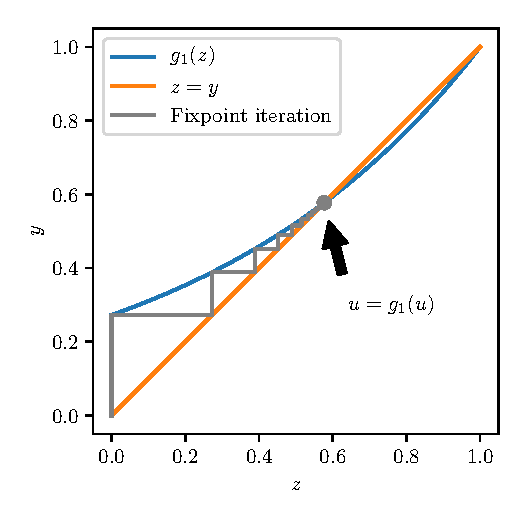
\includegraphics[scale=1]{u_solution_graphically.pdf}
	\caption{Graphical representation of eq. \eqref{Single layer u final} for an Erdos-Renyi network with $c = 1.3$. Gray solid line represent the successive steps of the fixpoint iteration.}
	\label{Figure: Solution of of u = g1(u) graphically}
\end{figure}

\subsection{Algorithm to find the connected components}

Since we are working in the limit of large $n$, the networks we are generating and analysing have large $n$ as well. Therefore the algorithm we use must be designed with some care to avoid consuming to much computing time, which would make them impractical to use. This motivate us to present the algorithm we use here.

To find all connected components of a network we proceed as follow
\begin{enumerate}
	\item Add all nodes to the set $\mathcal{S}\longsub{unprocessed}$ of unprocessed nodes.
	\item Remove one node from $\mathcal{S}\longsub{unprocessed}$ and add it to the set $\mathcal{S}\longsub{queued}$ of queued nodes.
	\item Start a new component $C$.
	\item Remove one node from $\mathcal{S}\longsub{queued}$ nodes and name it $v$.
	\item Add $v$ to the current component $C$.
	\item Add all unprocessed neighbors of $v$ to $\mathcal{S}\longsub{queued}$.
	\item If $\mathcal{S}\longsub{queued}$ is not empty go to 4, else store the component $C$ and continue.
	\item If $\mathcal{S}\longsub{unprocessed}$ is not empty go to 2, else terminate.
\end{enumerate}
This algorithm goes through each node exactly once and is thus of complexity $\bigO{n}$ which is the optimal complexity since all nodes must be associated to a component.

However, to ensure that the algorithm is fast we must be to efficiently find all neighbors of a node. To do that we represent the network as an \newconcept{adjacency list}: each node is given an index $i$ and the adjacency list $A_i$ contains all the neighbors of $i$. The whole network is thus represented as a list of adjacency list $A = (A_1, \dots, A_n)$.\footnote{For better performance during the creation of the network, our implementation goes a step further and actually request sorted adjacency lists.}

Other representation of networks exist, which are more convenient and efficient for some purposes. However we do not use them in this thesis and we stick to the adjacency list representation.

In fig. \ref{Figure: Single layer S simulation} we compare the fraction of the network occupied by the biggest component found using this algorithm with the numerical solution of eq. \eqref{Single layer S final} and \eqref{Single layer u final} computed using the fixpoint iteration \eqref{Single layer fixpoint g1 iteration}. As we can see the agreement between the two is very good for large $n$.

{\floatsetup[figure]{style=plain,subcapbesideposition=center}
\begin{figure}
	\sidesubfloat[]{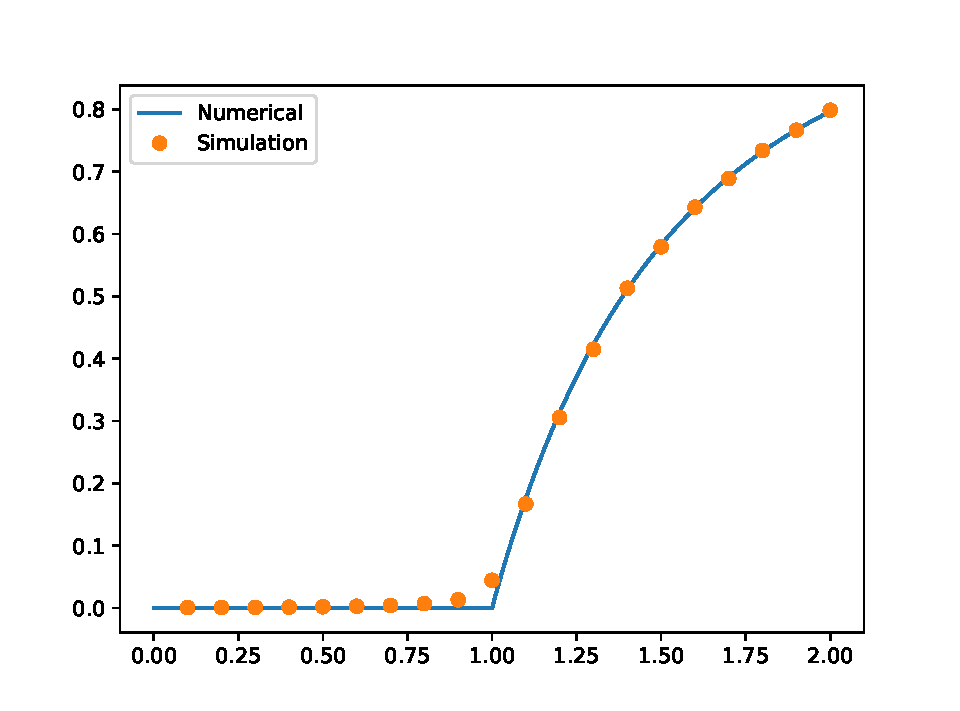
\includegraphics[width=0.8\textwidth]{numerical_simulation_one_layer_poisson.pdf}}\\
	\sidesubfloat[]{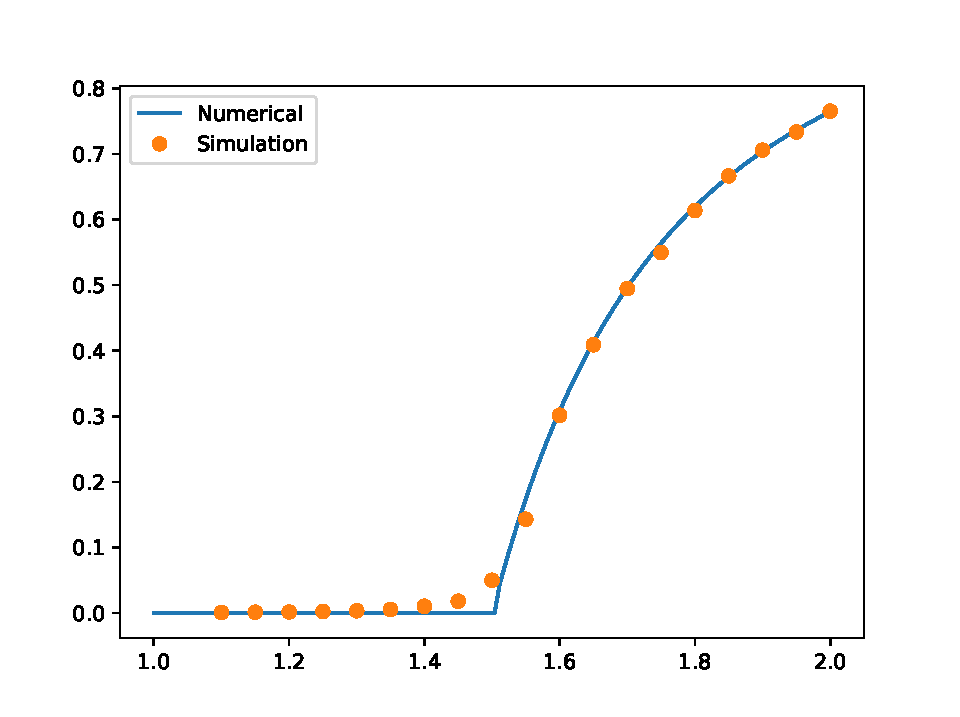
\includegraphics[width=0.8\textwidth]{numerical_simulation_one_layer_geometric.pdf}}
	\caption{Numerical solution of eqs. \eqref{Single layer S final} and \eqref{Single layer u final}, together with results on simulated networks. Results of simulations are average over 10 runs and the network size was set to $10^4$ nodes. Simulations ran for several seconds in total, indicating that much larger network should be easily usable. (A) Poisson degree distribution. (B) Geometric degree distribution.}
	\label{Figure: Single layer S simulation}
\end{figure}
}

\todo[inline]{Tidy the graphs and add scale-free}
\todo[inline]{Add graph with varying n to show the effect}

\subsection{Degree distribution in the GCC}
\label{Section: Degree distribution in the GCC}

Per Bayes theorem we have for two random events $A$ and $B$
\begin{align}
	P(A | B) = P(B | A) \frac{P(A)}{P(B)}. \label{Bayes theorem}
\end{align}
We can apply it to compute the probability $r_k$ that a vertex in the GCC has degree $k$
\begin{align}
	r_k &= P\left(\deg{v} = k | v \in GCC\right)\\
	&= P(v \in GCC | \deg{v} = k) \frac{P(\deg{v} = k)}{P(v \in GCC)} \\
	&= \frac{p_k}{S} \left(1 - P(v \notin GCC | \deg{v} = k)\right) =  \frac{p_k}{S} (1 - u^k). \label{Degree distribution in GCC}
\end{align}
To get the final result we used eq. \eqref{Probability that a node of degree k is not in the GCC}. This result was previously presented more generally and following a very different path in \cite{bauer2002maximal}.

Therefore we see that considering a vertex in the GCC biases the probability that it has degree $k$ by a factor $(1 - u^k)/S$ as compared to choosing a vertex uniformly in the network. Since both $u$ and $S$ are smaller than $1$, the net effect is to lower the proportion of low degree vertices in the GCC and thus to increase the proportion of high degree vertices. This result can be understood intuitively since in the configuration model the stubs are connected independently. Therefore each edge of a node increases the probability that this node is connected to the GCC, making high degree node over represented in the GCC.

\section{Generating connected networks}
\label{Section: Generating connected networks}

\subsection{Algorithm}

Algorithm previously in \cite{bialas2008correlations} \todo{Do something with with this information}

The knowledge of the degree distribution in the GCC can be used generate a connected component of a given degree distribution $r_k$ as follow: we first determine a degree distribution $p_k$ fulfilling eq. \eqref{Degree distribution in GCC} for some target degree distribution $r_k$. Then we generate a network with degree distribution $p_k$ using the configuration model. Finally we take its GCC as our connected network. By construction the vertices in the GCC will have degree distribution $r_k$. Determining the factors $p_k$ is not immediate however since $u$ is an unknown which is itself a function of $p_k$. We propose an algorithm to determine it numerically.

First we isolate $p_k$ from eq. \eqref{Degree distribution in GCC} to get
\begin{align}
	p_k &= S \pi_k(u), \quad \text{with} \quad \pi_k(z) = \frac{r_k}{1 - z^k}
\end{align}
Inserting this in the expression \eqref{Single layer u final} for $u$, we get
\begin{align}
	u &= \frac{\sum_{k=1}^\infty k \pi_k(u) u^{k-1}}{\sum_{k=1}^\infty k \pi_k(u)}. \label{Fixpoint equation for u}
\end{align}
Therefore $u$ is a fixpoint of the function
\begin{align}
	\mu(z) = \frac{\sum_{k=1}^\infty k \pi_k(z) z^{k-1}}{\sum_{k=1}^\infty k \pi_k(z)}, \label{Defition of mu}
\end{align}
which is fully determined by the GCC degree distribution $r_k$. Note that for $r_1 = 0$, we have the fixpoint $u = 0$ and $p_k = r_k$ for all $k$. This is consistent with the fact that small component of a network produced with the configuration model have a probability $0$ to have loop \cite{newman2010networks}. Indeed if $p_1 = 0$ all components must have loops, therefore the probability to have small components is $0$ as well.

On the other hand $r_1 > 0$ implies $u > 0$. To approximate its value we define the sequence $u_{j+1} = \mu(u_j)$, with $u_0 = r_1$. This sequence will converge toward $u$ for large $j$. A proof of this statement is given in Appendix \ref{Appendix: Fixpoint convergence}.

In practice we can not deal evaluate infinite sums numerically, thus we need to choose a cutoff index $K$ for the sums such that
\begin{align}
	\sum_{k=K+1}^\infty k \pi_k(u) \ll 1.
\end{align}
For scale-free network with exponent smaller than 2 for example, this sum always diverges and thus this method is not applicable.

Once $u$ is approximated, we can compute the first $K$ probabilities $p_k$, which is sufficient to sample random numbers between $1$ and $K$ with relative probability $p_k$. If $K$ is chosen such that $r_k << 1$ for $k > K$, the degree distribution in the GCC closely approximate the distribution $r_k$.

\subsection{Erdos-Renyi reconstruction}

In order to test the algorithm presented, we choose the target connected degree distribution $r_k$ to be the degree distribution of the GCC of an Erdos-Renyi network. It is then expected that the reconstructed $p_k$ closely approximate a Poisson degree distribution.

The probability $p_k$ to have degree $k$ in an Erdos-Renyi network is given in eq. \eqref{pk for Erdos-Renyi}. Using eq. \eqref{Single layer u final} and \eqref{Single layer S final} to find $u$ and $S$ yield everything we need to be able to determine the GCC degree distribution $r_k$ from eq. \eqref{Degree distribution in GCC}. We can therefore use the algorithm on these $r_k$.

When computing $S$ for the original Poisson distribution, we should however be cautious, as the reconstructed $p_0$ will always be $0$. The expected resulting degree distribution, correctly normalized, is therefore
\begin{align}
	p_k = \frac{c^k}{k!} \frac{1}{e^{c} - 1}.
\end{align}
The expected bias ratio $r_k/p_k$ is shown for various mean degree $c$ and a cutoff constant $K = 10000$ in fig. \ref{Figure: Erdos-Renyi reconstruction} together with the same value computed from the algorithm presented above. As it can be seen, the agreement is very good. During the computations it has been observed that the closer the mean degree is to the critical value $c = 1$, the slower the fixpoint iteration converges.

\begin{figure}
	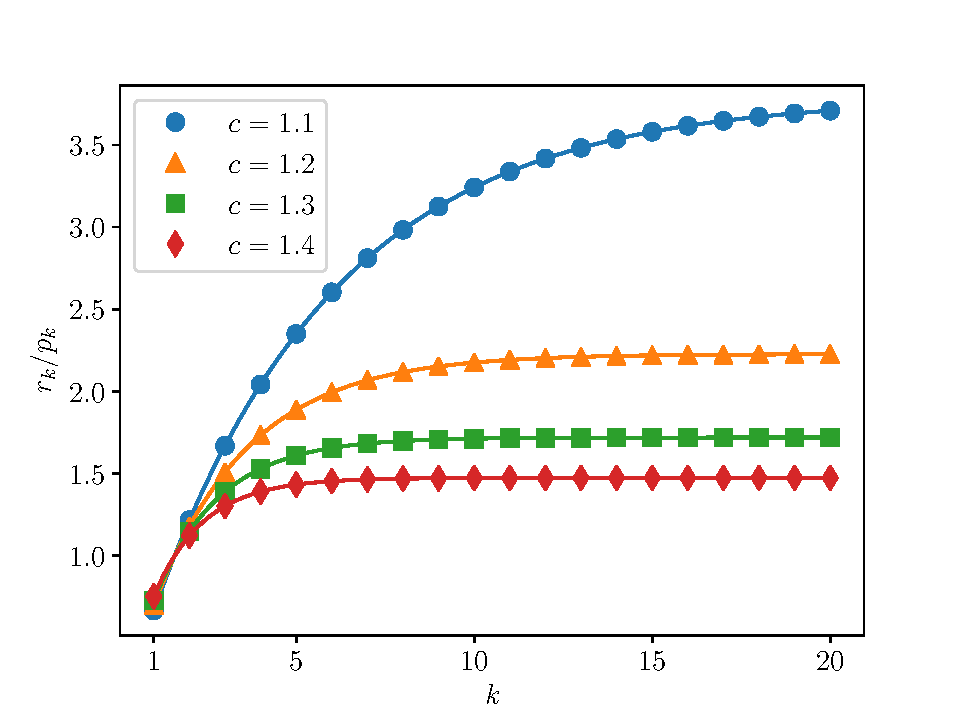
\includegraphics[width=0.8\textwidth]{ER_reconstruction.pdf}
	\caption{Bias factor $r_k/p_k$ for $r_k$ being the degree distribution of the GCC of an Erdos-Renyi network with various mean degree $c$ and cutoff constant $K = 10000$. The $p_k$ have been determined using the algorithm presented in the text. Solid line is the expected value $(1 - u^k)/S$ for the bias factor.}
	\label{Figure: Erdos-Renyi reconstruction}
\end{figure}

\subsection{Real world networks}

As an example of use of the algorithm presented, we apply it to real networks. We choose two by design connected network from the Konect network database \cite{kunegis2013konect}, the powergrid of the western states of the United States and the road network of the state of California\footnote{The codes of the networks in the Konect database are respectively \code{UG} and \code{RO}.}.

The connected degree distribution $r_k$ is taken to be the empirical degree distribution of the real network considered. As a consequence, the cutoff constant $K$ is the maximal degree appearing in the network. Then, to sample the resulting degree distribution $p_k$, we simply take the number of vertex $d_k$ of degree $k$ to be the closest integer to $n p_k$, where $n$ is the total number of nodes. In the examples presented we use $n = 10^7$.

\begin{figure}
	\sidesubfloat[]{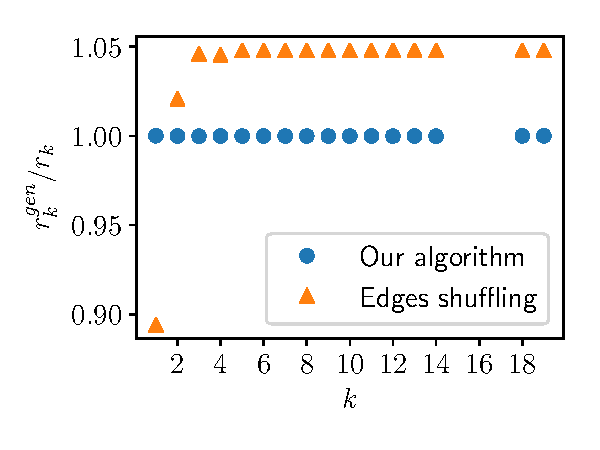
\includegraphics[width=0.45\textwidth]{real_US-power-grid.pdf}}\hfill
	\sidesubfloat[]{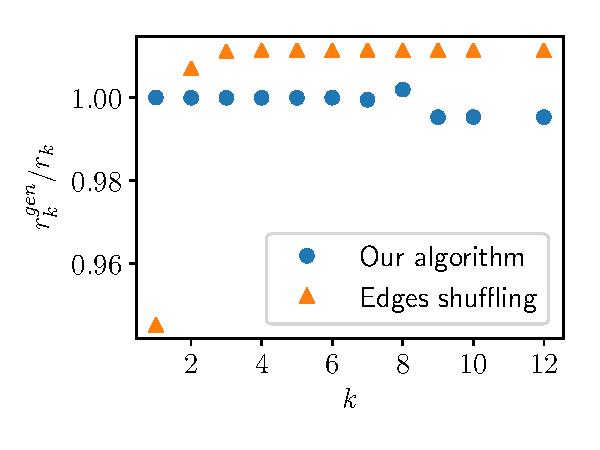
\includegraphics[width=0.45\textwidth]{real_roadNet-CA.pdf}}
	\caption{Plot of the ratio of the generated connected degree distribution $r^{gen}_k$ to the target degree distribution $r_k$ taken from a real network for our algorithm and the edges shuffling method. Missing values correspond to degree with probability $0$ to appear. (A) Western US power-grid network. (B) California road network.}
	\label{Figure: Real examples}
\end{figure}

We compare the degree distribution $r^{gen}_k$ of the GCC of the newly generated network with the target distribution $r_k$ by looking at the ratio $r^{gen}_k / r_k$. Resulting ratios are shown in fig. \ref{Figure: Real examples}, together with the results obtained by taking the GCC of the reshuffled network.


\chapter{Multiplex networks}
\label{Section: Multiplex networks}

\section{Introduction}

\todo[inline]{Move this to the general introduction ? Put the actual general introduction into the single layer network chapter ?}

The concept of network can be extended by allowing different types of edges between the nodes of a network. Such generalized networks are called \newconcept{multiplex networks} or \newconcept{multi layers networks}. Real world example of such multiplex networks are numerous, for example there are many different types of connections between cities: transport connections (road, railroads, airlines), information connections (phone lines, internet connections) or supply connections (electricity, water).

Mathematically, it is convenient to represent multiplex networks in a slightly different but equivalent way. We consider each type of edge to generate its own network. If we started with $L$ different type of edges, we therefore get $L$ networks, all sharing the same set of nodes. Conceptually it is similar to stack $L$ networks on top of each other, each network forming a \newconcept{layer} of the composed multi layers network (hence the name). An illustration of both representation of multiplex networks is shown in fig. \ref{Figure: Representations of multiplex networks} for a two layers network.

\begin{figure}
	
\sidesubfloat[]{
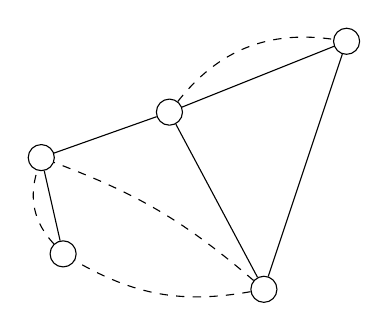
\begin{tikzpicture}[y=-1cm, scale=1.5]

	\node[node] (A) at (0.2, 0) {} ;
	\node[node] (B) at (1, 1.5) {} ;
	\node[node] (C) at (-0.7, 1.2) {} ;
	\node[node] (D) at (-0.5, -0,1) {} ;
	\node[node] (E) at (1.7, -0.6) {} ;

	\draw (A) -- (B) ;
	\draw (A) -- (D) ;
	\draw (A) -- (E) ;
	\draw (B) -- (E) ;
	\draw (C) -- (D) ;
	
	\draw[dashed] (A) to[bend left] (E) ;
	\draw[dashed] (B) to[bend left=20] (C) ;
	\draw[dashed] (B) to[bend right=10] (D) ;
	\draw[dashed] (C) to[bend left] (D) ;
\end{tikzpicture}
}\hspace{1cm}
\sidesubfloat[]{
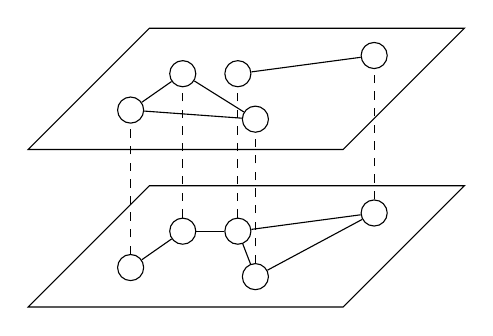
\begin{tikzpicture}[y = 2cm]
	\node[node] (A) at (0.2, 0, 0) {} ;
	\node[node] (B) at (1, 0, 1.5) {} ;
	\node[node] (C) at (-0.7, 0, 1.2) {} ;
	\node[node] (D) at (-0.5, 0, -0,1) {} ;
	\node[node] (E) at (1.7, 0, -0.6) {} ;
	
	\node[node] (A') at (0.2, 1, 0) {} ;
	\node[node] (B') at (1, 1, 1.5) {} ;
	\node[node] (C') at (-0.7, 1, 1.2) {} ;
	\node[node] (D') at (-0.5, 1, -0,1) {} ;
	\node[node] (E') at (1.7, 1, -0.6) {} ;
	
	\draw (-1.5, 0, -1.5) -- (2.5, 0, -1.5) -- (2.5, 0, 2.5) -- (-1.5, 0, 2.5) -- cycle ;
	\draw (-1.5, 1, -1.5) -- (2.5, 1, -1.5) -- (2.5, 1, 2.5) -- (-1.5, 1, 2.5) -- cycle ;
	
	\foreach \p in {A, B, C, D, E}
	{
		\draw[dashed] (\p) -- (\p') ;
	}
	
	\draw (A) -- (B) ;
	\draw (A) -- (D) ;
	\draw (A) -- (E) ;
	\draw (B) -- (E) ;
	\draw (C) -- (D) ;
	
	\draw (A') -- (E') ;
	\draw (B') -- (C') ;
	\draw (B') -- (D') ;
	\draw (C') -- (D') ;
	
	
\end{tikzpicture}
}
	\caption{Possible representations of a two layers network. (A) A network with two kinds of edges, straight solid edges and curved dashed ones. (B) Two networks in separate layers with corresponding nodes.}
	\label{Figure: Representations of multiplex networks}
\end{figure}

Thinking in term of layers allows to reuse all quantities define in the context of single layer networks, such as the generating functions. We the extended quantity the same way as the original one, adding a subscript $i$ to its symbol to denote the fact that it applies to layer $i$, except if the symbol already has a subscript. In this case we add a superscript $(i)$.

Finally, we only consider that each layer of a multiplex network is independant to each other. This is most likely not true for real networks, but we restrict ourself to this case for simplicity.

\section{Giant viable cluster}

\subsection{Size of the GVC}

For single layer network, we are interested in the GCC as it is common for a system to be operational only if it is connected to the whole corresponding network. In the context of multiplex networks, the concept of connected component is extended by introducing \newconcept{viable clusters}. A viable cluster is defined as a subset of the multiplex network in which there is a path between each pair of vertices in all layers. Note that the path between two vertices must be totally included in the viable cluster. As a consequence, the intersection of connected components is not in general a viable clusters as it is illustrated in fig. \ref{Figure: Intersection of connected is not viable}.

\begin{figure}
	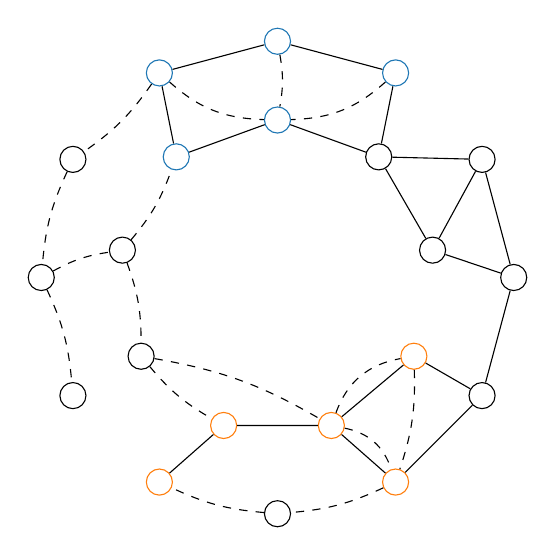
\begin{tikzpicture}
	\foreach \n in {1, 2, ..., 9}
	{
		\node (C\n') at ({2*sin(\n*360/9)}, {2*cos(\n*360/9)}) {} ;
	}
	
	
	\foreach \n in {1, 2, ..., 12}
	{
		\node (D\n') at ({3*sin(\n*360/12)}, {3*cos(\n*360/12)}) {} ;
	}
	
	\foreach \p in {D11, D12, D1, C8, C9}
	{
		\node[node, color=C0] (\p) at (\p') {} ;
	}
	
	\foreach \p in {C3, C4, C5, D5, D7}
	{
		\node[node, color=C1] (\p) at (\p') {} ;
	}
	
	\foreach \p in {C1, C2, C6, C7, D2, D3, D4, D6, D8, D9, D10}
	{
		\node[node] (\p) at (\p') {} ;
	}
	
	\draw (D7) -- (C5) -- (C4) -- (C3) -- (D4) -- (D5) -- (C4) ;
	\draw (D4) -- (D3) -- (D2) -- (C2) -- (D3) ;
	\draw (C2) -- (C1) -- (D2) ;
	\draw (C1) -- (D1) -- (D12) -- (D11) -- (C8) -- (C9) -- (C1) ;
	
	\draw[dashed] (D1) to[bend left=20] (C9) ;
	\draw[dashed] (D12) to[bend left=10] (C9) ;
	\draw[dashed] (D11) to[bend right=20] (C9) ;
	\draw[dashed] (D11) to[bend left=10] (D10) ;
	\draw[dashed] (D10) to[bend right=10] (D9) ;
	\draw[dashed] (D9) to[bend left=10] (D8) ;
	\draw[dashed] (D9) to[bend left=10] (C7) ;
	\draw[dashed] (C7) to[bend right=10] (C8) ;
	\draw[dashed] (C7) to[bend left=10] (C6) ;
	\draw[dashed] (C6) to[bend left=10] (C4) ;
	\draw[dashed] (C4) to[bend left] (C3) ;
	\draw[dashed] (C4) to[bend left] (D5) ;
	\draw[dashed] (C3) to[bend left=10] (D5) ;
	\draw[dashed] (D5) to[bend left=10] (D6) ;
	\draw[dashed] (D6) to[bend left=10] (D7) ;
	\draw[dashed] (C6) to[bend right=10] (C5) ;
\end{tikzpicture}
	\caption{Intersection of connected components of two layers of a multiplex networks, represented respectively with solid straight line and with curved dashed line. The intersection is composed of the colored nodes, however there is no path in the intersection connecting the blue and orange nodes. Therefore the intersection results in two distinct viable clusters.}
	\label{Figure: Intersection of connected is not viable}
\end{figure}

\todo[inline]{Correct the following explanation, it is going nowhere}
The rationale behing this definition can be clarified by the introduciton of the \newconcept{giant viable cluster} (GVC) which is the extension of the single layer concept of GCC, i.e. a viable cluster which occupy a non zero fraction of the whole network in the limit of large $n$. Let consider that a node is functional only if it is connected to the GVC. One example of such requirement is the network of powergrid regulation stations\todo{Find a ref ?}. Such stations must be connected to both the powergrid and an internal

Let $g_0^{(i)}$ and $g_1^{(i)}$ be the generating functions of respectively the degree and the excess degree distribution in layer $i$. Moreover define $u_i$ as the probability that a vertex reached after following an edge in layer $i$ is not part of the giant viable cluster. Be aware that $u_i$ is not the direct extension of the single layer $u$ quantity, which correspond to the probability not to be part of the GCC.

Then if we pick a vertex $v$ at random the probability $S$ that it is part of the giant viable cluster can be written as
\begin{align}
	S &= P_0\left(\bigcap_{i = 1}^{L} \exists w \in N_i(v) \; w \in GVC \right).
\end{align}
By requiring that the layers are independent from one others, we can rewrite $S$ as a product
\begin{align}
	S &= \prod_{i = 1}^{L}  P_0^{(i)}\left(\exists w \in N_i(v) \; w \in GVC\right) \\
		&=\prod_{i = 1}^{L}  \left[1 - P_0^{(i)}\left(w \notin GVC \; \forall w \in N_i(v)\right) \right] \\
		&=\prod_{i = 1}^{L}  \left[1 - \sum_{k = 0}^{\infty} P_0^{(i)}\left(w \notin GVC \; \forall w \in N_i(v) | \deg{v} = k \right) p^{(i)}_k \right] \\
		&=\prod_{i = 1}^{L}  \left[1 - \sum_{k = 0}^{\infty} P_1^{(i)}\left(v \notin GVC | \deg{v} = k \right) p^{(i)}_k \right] \\
		&=\prod_{i = 1}^{L}  \left[1 - \sum_{k = 0}^{\infty} u_i^k p^{(i)}_k \right] \\
		&=\prod_{i = 1}^{L}  \left[1 - g_0^{(i)}(u_i) \right].\label{Multiplex GCC size final}
\end{align}

We can find $u_j$ by a similar reasoning. First note that $1 - u_j$ is the probability that a vertex reached by following an edge in layer $j$ is in the giant viable cluster. Which as before can be written in the form
\begin{align}
	1 - u_j &= P_1^{(j)}\left(\bigcap_{i = 1}^{L} \exists w \in N_i(v) \; w \in GVC\right)\\
	&= \prod_{i = 1}^{L}  P_1^{(j)}\left(\exists w \in N_i(v) \; w \in GVC \right).
\end{align}
Since the layers are independent, the fact that we reached $v$ by following an edge in layer $j$ to reach vertex $v$ is irrelevant in all other layers. However in layer $j$ this means that the degree distribution follows the distribution $q_k^{(j)}$ rather than $p_k^{(j)}$. Putting this together we get
\begin{align}
	1 - u_j &= \left[1 - \sum_{k = 0}^{\infty} u_j^k q_k^{(j)} \right] \prod_{\substack{i = 1 \\ i \neq j}}^{L}  \left[1 - \sum_{k = 0}^{\infty} u_i^k p^{(i)}_k \right] \\
	&= \left[1 - g_1^{(j)}(u_j) \right] \prod_{\substack{i = 1 \\ i \neq j}}^{L}  \left[1 - g_0^{(i)}(u_i) \right]. \label{Multiplex u final}
\end{align}

{\floatsetup[figure]{style=plain,subcapbesideposition=center}
\begin{figure}
	\sidesubfloat[]{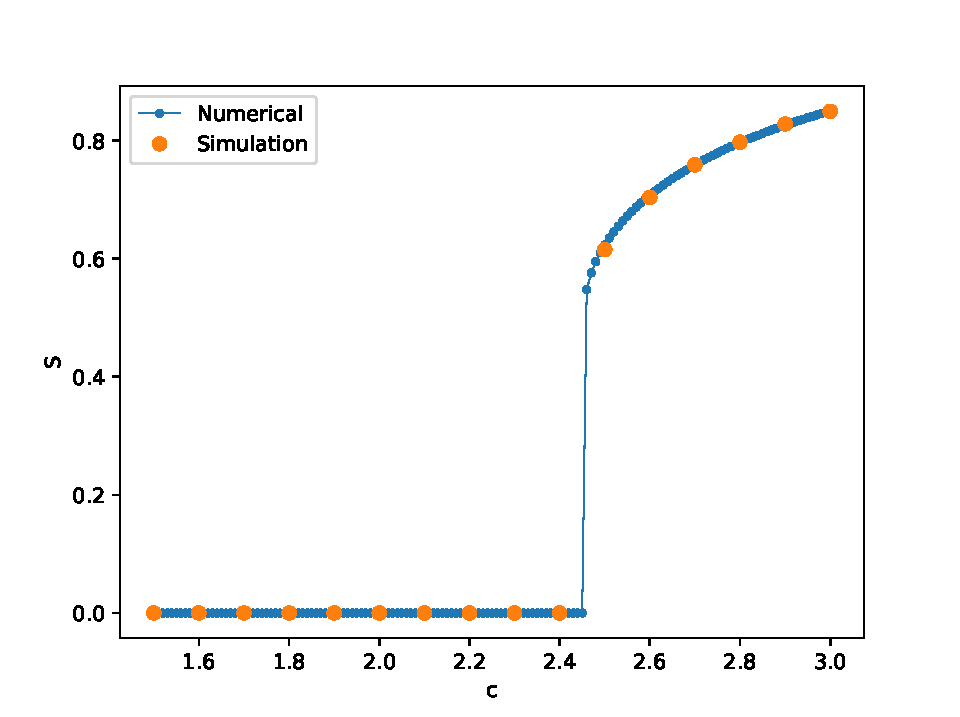
\includegraphics[width=0.8\textwidth]{numerical_simulation_double_layer_poisson_equal_c.pdf}}\\
	\sidesubfloat[]{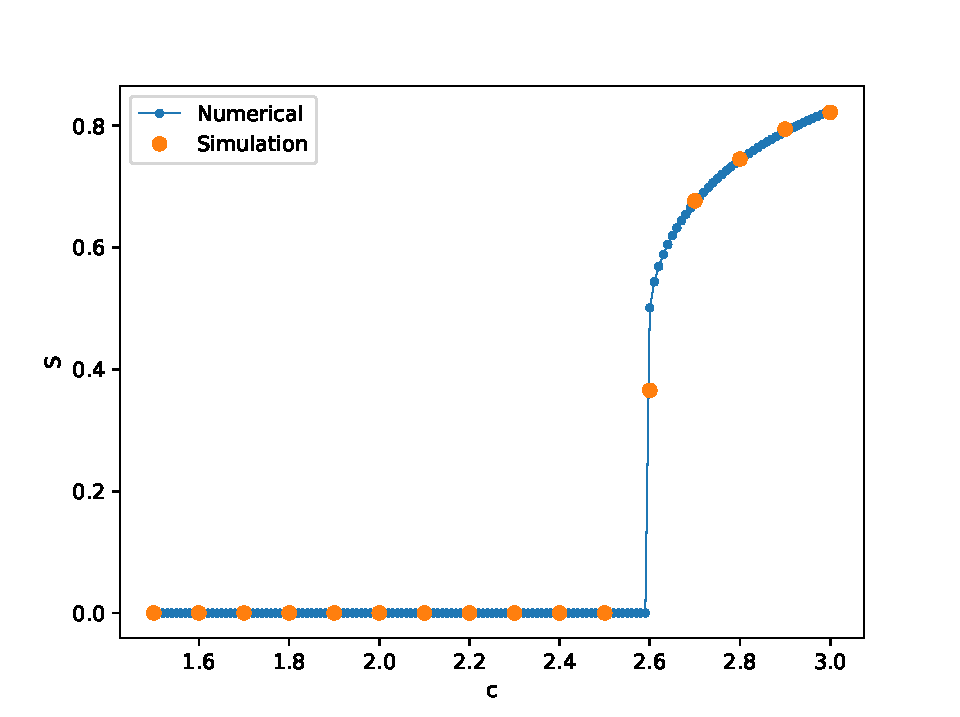
\includegraphics[width=0.8\textwidth]{numerical_simulation_double_layer_geometric_equal_c.pdf}}
	\caption{Numerical solution of eqs. \eqref{Multiplex GCC size final} and \eqref{Multiplex u final}, together with results on simulated networks for multiplex networks composed of two layers with the same distribution and mean number of edge $c$. Results of simulations are average over 10 runs and the network size was set to $10^4$ nodes. Simulations ran for several seconds in total, indicating that much larger network should be easily usable. (A) Poisson degree distribution. (B) Geometric degree distribution.}
\end{figure}
}


\subsection{Algorithm to find the viable clusters}
\todo[inline]{Write. Make sure to introduce small components problem}

\section{Boundary condition}

\todo[inline]{Write some introduction}

Up to now, we have considered the multiplex generated to be determined via the degree distributions of each of its layer. However a degree distribution has an infinite number of degrees of freedom, therefore it is more practical to let the degree distributions depend on a finite set of parameters $\lambda_1, \lambda_2, \dots, \lambda_N$ and express the behaviour of the network in term of them. Note that the number of parameters $N$ does not need to match the number of layers $L$.

In order to make our main statement about the critical region for a multiplex network, we need to introduce several quantities. First, let introduce
\begin{align}
	\uvec &= (u_1, u_2, \dots, u_L) \\
	\lambdavec &= (\lambda_1, \lambda_2, \dots, \lambda_N) \\
	f_j(\lambdavec, \uvec) &= 1 - u_j - \left[1 - g_1^{(j)}(u_j) \right] \prod_{\substack{i = 1 \\ i \neq j}}^{L}  \left[1 - g_0^{(i)}(u_i) \right] \label{Definition fj}
\end{align}
and the function
\begin{align}
	F : \mathbb{R}^N \times \unitinterval^L &\rightarrow \mathbb{R}^L \\
	(\lambdavec, \uvec) &\mapsto F(\lambdavec, \uvec) = (f_1(\lambdavec, \uvec), f_2(\lambdavec, \uvec), \dots, f_L(\lambdavec, \uvec)), \label{Definition F}
\end{align}
where $\unitinterval = [0, 1]$. The variables $\uvec$ in which we are interested are always in $\unitinterval^L$, since $u_i$ represents a probability for all $i$.

Since the functions $g_0^{(i)}$ and $g_1^{(i)}$ are analytic with respect to the $u_i$, the function
\begin{align}
	F_{\lambdavec} : \unitinterval^L &\rightarrow \mathbb{R}^L\\
		\uvec &\mapsto F_{\lambdavec}(\uvec) = F(\lambdavec, \uvec),
\end{align}
is continuously differentiable for all parameters $\lambdavec$. Therefore we can define Jacobi matrix $J(\lambdavec, \uvec)$ of $F_{\lambdavec}$ as having coefficients
\begin{align}
	\left[ J(\lambdavec, \uvec) \right]_{ij} = \frac{\partial f_i(\lambdavec,\uvec)}{\partial u_j}.
\end{align}

With the help of the notation introduced, we can now express solving eq. \eqref{Multiplex u final} as being equivalent to finding $\uvec^* \in \unitinterval^L$ such that
\begin{align}
	F(\lambdavec, \uvec^*) = 0. \label{Implicit equation}
\end{align}
If this equation only admits the trivial solution $\uvec^* = \uvec_T$, the parameter $\lambdavec$ corresponds to a state without GVC. On the other if multiple solutions $\uvec^*$ exist, a GVC must exist as well. To determine the boundary between these two regions (i.e. the critical region), we use the implicit function theorem.

First, we assume that $F$ (and not only $F_{\lambdavec}$) is continuously differentiable and that we know a solution $\uvec^*$ of \eqref{Implicit equation} for some parameter vector $\lambdavec^*$. With that assumption the implicit function theorem can be state as follow:

If $\det\left[ J(\lambdavec^*, \uvec^*) \right] \neq 0$ then there is an open neighbourhood $U \subset \mathbb{R}^L$ of $\lambdavec^*$ such that there is an unique continuously differentiable function $h : U \rightarrow \unitinterval^L$ with
\begin{align}
	h(\lambdavec^*) &= \uvec^* \\
	F(\lambdavec, h(\lambdavec)) &= 0, \quad \forall \lambdavec \in U. \label{Implicit solution for F}
\end{align}

The result in which we are interested here comes from the contrapositive of this statement, namely that if for all neighbourhoods $U$ we can not find a uniquely defined continuous function $h$, then the determinant of the Jacobi matrix $J(\lambdavec, \uvec)$ must be zero,
\begin{align}
	\det\left[ J(\lambdavec^*, \uvec^*) \right] = 0 \label{Boundary condition}.
\end{align}
This condition has previously been outlined, without proof in \cite{baxter2012avalanche}. We now prove that such situations arise if $\lambdavec^*$ is a critical point of the phase transition between the absence and existence of a GVC, and therefore that eq. \eqref{Boundary condition} is a sufficient condition to find the critical region of such phase transition.

First notice that in the context of multiplex network a phase transition appears between the trivial solution $\uvec_T = (1, 1, \dots, 1)$ (where $S = 0$) and non trivial solutions ($S > 0$). However, the trivial solution $\uvec_T$ solves eq. \eqref{Multiplex u final} for any generating function and thus for any parameter vector $\lambdavec$. For a continuous phase transition this immediately gives us $\uvec^* = \uvec_T$. Moreover, on one side of the phase transition occurring at $\lambdavec^*$ one solution exists, while on the other at least two do. Therefore for any $U$ open containing $\lambdavec^*$ we can define two distinct functions on $U$ that fulfil eq. \eqref{Implicit solution for F}, the trivial $h_T(\lambdavec) = \uvec_T$ and another function $h$ corresponding to the non trivial solutions, with $h(\lambdavec^*) = h_T(\lambdavec^*) = \uvec_T$. So the function $h$ of the implicit function theorem is not uniquely defined and thus $\det\left[ J(\lambdavec^*, \uvec_T) \right] = 0$.

\begin{figure}
	\sidesubfloat[]{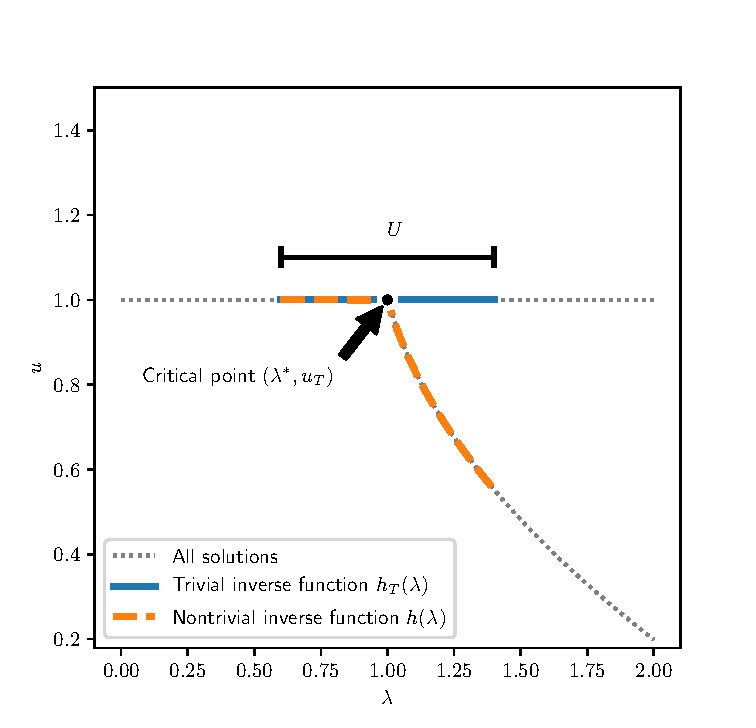
\includegraphics[height=0.35\textwidth]{scheme_continuous_phase_transition}}\hfill
	\sidesubfloat[]{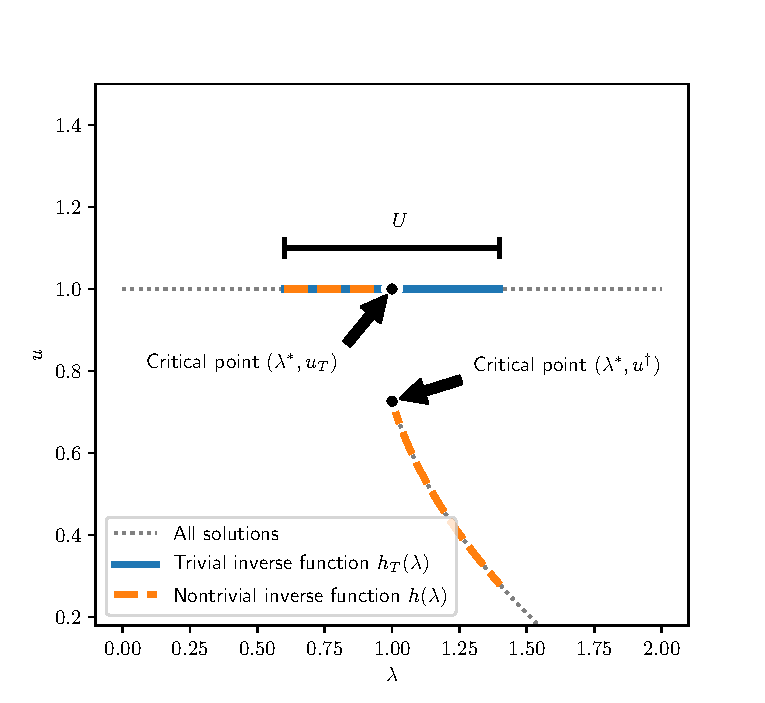
\includegraphics[height=0.35\textwidth]{scheme_discontinuous_phase_transition}}
	\caption{(a) Scheme of a continuous phase transition. (b) Scheme of a discontinuous phase transition.}
	\label{Figure: Scheme of continuous and discontinuous phase transitions}
\end{figure}

On the other hand, let consider a discontinuous phase transition at $\lambdavec^*$. For any neighbourhood $U$ of $\lambdavec^*$ there are two sequences $(\lambdavec_n, \uvec_n)$ and $(\etavec_m, \vvec_m)$ with $\lambdavec_n, \etavec_m \in U$ such that
\begin{align}
	\lim_{n \rightarrow \infty} (\lambdavec_n, \uvec_n) &= (\lambdavec^*, \uvec^\dagger) \quad \text{ avec } \uvec^\dagger \neq \uvec_T \\
	\lim_{m \rightarrow \infty} (\etavec_m, \vvec_m) &= (\lambdavec^*, \uvec_T) \\
	F(\lambdavec_n, \uvec_n) &= 0 \quad \forall n \\
	F(\etavec_m, \vvec_m) &= 0 \quad \forall m.
\end{align}
If we assume that an unique continuous function $h$ solving eq. \eqref{Implicit solution for F} exists, we would have
\begin{align}
	h(\lambdavec_n) &= \uvec_n \quad \forall n \\
	h(\etavec_m) &= \vvec_m \quad \forall m.
\end{align}
The continuity of $h$ would furthermore imply
\begin{align}
	h(\lambdavec^*) = \lim_{n \rightarrow \infty} h(\lambdavec_n) = \lim_{n \rightarrow \infty} \uvec_n = \uvec^\dagger,
\end{align}
but also
\begin{align}
	h(\lambdavec^*) &= \lim_{m \rightarrow \infty} h(\etavec_m) = \lim_{m \rightarrow \infty} \vvec_m = \uvec_T.
\end{align}
Since $\uvec_T \neq \uvec^\dagger$, this gives raise to the contradiction $h(\lambdavec^*) \neq h(\lambdavec^*)$. Therefore our assumption must be false and no continuous function $h$ can be defined to solve eq. \eqref{Implicit solution for F}. So finally, we have $\det\left[ J(\lambdavec^*, \uvec^*) \right] = 0$, $\uvec^*$ being either $\uvec_T$ or $\uvec^\dagger$.

If $L = N = 1$, the problem simplifies to the single layer case in which the degree distribution is determined by a single parameter $\lambda$. In that case the Jacobi matrix $J$ reduces to the scalar quantity
\begin{align}
	J(\lambda, u) = \frac{\partial}{\partial u} \left(g_1(u) - u\right) = \frac{\partial g_1(u)}{\partial u} - 1.
\end{align}
Therefore the condition for the boundary $\det J(\lambda, u) = 0$ becomes
\begin{align}
	\frac{\partial g_1(u)}{\partial u} = 1.
\end{align}
This condition correctly reduces to the one given previously in eq. \eqref{Boundary condition for single layer}.

\section{Interval estimation of the critical region}

\subsection{Motivation}

In order to verify that eq. \eqref{Boundary condition} indeed gives the critical region for a multiplex network, we need to introduce an independent numerical method to approximate it. This comes down to find the number of solutions of eq. \eqref{Multiplex u final} in the whole parameter space and then draw the boundary of the regions with a constant number of solution. However this leads to two problems.

First, standard algorithms to find zeros of functions do not guarantee that all zeros are found. These algorithms usually found one solution at a time, the one being found depending on the initial guess solution provided by the user. This causes immediate problem for our purpose, since missing a solution of eq. \eqref{Multiplex u final} may drastically change our estimation of the boundary region.

Secondly, the standard algorithms can only deal with one point of the parameter space at a time. This forces us to restrict our search on a discrete set of parameters. If this set is ill chosen, we may miss important features of the critical region.

The second point is minor compare to the first. We indeed expect the critical region to be smooth and therefore restricting our analysis on any lattice should reasonably approximate it. We still mention this caveat however, since it can be solved by the same method as the first one, namely by introducing \newconcept{interval arithmetic}. Interval arithmetic is a framework, presented in the next section, that allows to guarantee under some circumstance that all zeros of a function have been found and to work with regions of the parameter space rather than discrete points.

\subsection{Interval arithmetic}

Let $C \subset \mathcal{R}^L$ be the set of all parameters $\lambdavec$ corresponding to a critical point. This set correspond to the parameters that solve simultaneously eq. \eqref{Multiplex u final} and eq. \eqref{Boundary condition} for some $\uvec \in \unitinterval^L$. 

First of all an \newconcept{interval} $I$ is defined a set of the form
\begin{align}
	I = \interval{a, b} = \set{x \in \mathbb{R} | a \leq x \leq b}.
\end{align}
The set of all intervals is denoted as $\mathbb{IR}$. The $N$-dimensional equivalent of an interval is an \newconcept{interval box} $B$, defined as the Cartesian product of $N$ intervals,
\begin{align}
	B = I_1 \times I_2 \times \cdots \times I_N, \quad I_k \in \mathbb{IR} \quad \forall k = 1, \dots, N
\end{align}
The set of all $N$-dimensional interval boxes is denoted $\mathbb{IR}^N$.

Given a function $\phi : \mathbb{R}^M \rightarrow \mathbb{R}^N$ we define a new interval valued function $\Phi : \mathbb{IR}^M \rightarrow \mathbb{IR}^N$ such that
\begin{align}
	x \in B \quad \Rightarrow \quad \phi(x) \in \Phi(B). \label{Definition interval extension}
\end{align}
A function $\Phi$ with this property is called an \newconcept{interval extension} of $\phi$. In other words $\Phi(B)$ is guaranteed to contains all possible image of $B$ under $\phi$. Note that an interval extension is not unique, and we would like to use the \emph{tightest} possible extension, meaning that we want $\Phi(B)$ to approximate $\phi(B)$ as closely as possible. A perfect estimation is however not possible in general since the image of an interval box is not always itself an interval box.

Note that as oppose to $\phi$, its interval extension $\Phi$ is exactly representable numerically. This can be done by requiring the fact that the implementation of $\Phi$ includes numerical inaccuracy in such a way that the eq. \eqref{Definition interval extension} holds for the finite precision numerical result $\Phi(B)$. Hopefully good implementations, that respect this condition and are reasonably tight, can be found in existing libraries. In this thesis we use the implementation provided by the Julia package \code{IntervalArithmetic.jl}\missingref{}.

The next step is to solve eq. \eqref{Multiplex u final}. Several general schemes exist to solve equations in a guaranteed way using interval arithmetic\missingref{}, but here we use a simpler algorithm inspired by them and more suited to our present needs.

We define
\begin{align}
	\psi(\lambdavec, \uvec) = F(\lambdavec, \uvec) + \uvec,
\end{align}
with components
\begin{align}
	\psi_j(\lambdavec, \uvec) = 1 - \left[1 - g_1^{(j)}(u_j) \right] \prod_{\substack{i = 1 \\ i \neq j}}^{L}  \left[1 - g_0^{(i)}(u_i) \right].
\end{align}
Also we define $\Psi$ as an interval extension of $\psi$.

Now, let $\uvec^* \in U_0$ be a solution of \eqref{Implicit equation} for some $\lambdavec \in \Lambda$. By the definition of $\psi$ and eq. \eqref{Definition interval extension},
\begin{align}
	F(\lambdavec^*, \uvec^*) = 0 \quad \Rightarrow \quad \uvec^* = \psi(\lambdavec^*, \uvec^*) \in \Psi(\Lambda, U_0).
\end{align}
Therefore if we apply $\Psi(\Lambda, \cdot)$ to an interval box $U_0$ containing a solution, the resulting interval box contains the solution as well. We know that all solutions $\uvec^*$ are contained in $\unitinterval$ by definition of $\uvec$ and thus by iterating the previous argument from $U_0 = \unitinterval$, all solutions are elements of the interval boxes $U_k(\Lambda)$ recursively defined by
\begin{align}
	U_{k+1}(\Lambda) = \Psi(\Lambda, U_k(\Lambda)). \label{Recursion relation for Uk}
\end{align}
Therefore if we find $k$ such that $U_k = \set{\uvec_T}$, we know that the system for any $\lambdavec \in \Lambda$ only admits the trivial solution.

In practice however, the sequence $U_k$ never converges to exactly the set $\set{\uvec_T}$, we therefore consider the criterion to be met if
\begin{align}
	U_k \subset [1 - \varepsilon, 1]^L, \label{Criterion for trivial region}
\end{align}
for some small tolerance $\varepsilon$.

Furthermore it is possible in some cases to guarantee the presence of non trivial solutions, allowing to conclude that a GVC emerges. Indeed, if we can find some interval boxes $\Lambda$ and $U$ such that
\begin{align}
	\Psi(\Lambda, U) \subset U \quad \text{and} \quad \uvec_T \notin U, \label{Criterion for non trivial solution}
\end{align}
then by definition of the interval extension (eq. \eqref{Definition interval extension}), we have
\begin{align}
	\psi(\lambdavec, U) \subset U, \quad \forall \lambdavec \in \Lambda.
\end{align}
Since $U$ is closed and simply connected, the fixpoint theorem \todo{Find back which one exactly}\missingref{} applies, implying that for each $\lambdavec \in \Lambda$ there must be at least one $\uvec^*$ in $U$ such that $\uvec^*$ is a fixpoint, or in other words such that $\uvec^* = \psi(\lambdavec, \uvec^*)$. Therefore eq. \eqref{Criterion for non trivial solution} is a sufficient condition to prove the existence of at least one solution. Moreover since we imposed $\uvec_T \notin U$, the solution present can not be the trivial one.

\subsection{Algorithm}

Equations \eqref{Criterion for trivial region} and \eqref{Criterion for non trivial solution} give guaranteed criteria for respectively the absence and presence of a non trivial solution in the region $\Lambda$ considered. This is sufficient to propose an algorithm to estimate the critical region $C$.

\begin{enumerate}
	\item Choose an initial parameter region and store it in the set $\mathcal{S}\longsub{working}$ of regions yet to be processed.
	\item If $\mathcal{S}\longsub{working}$ is empty terminate, otherwise retrieve the next parameter region from $\mathcal{S}\longsub{working}$, and call it $\Lambda$.
	\item If the radius of $\Lambda$ is smaller than some tolerance $\delta$, store it in the set $\mathcal{S}\longsub{unkown}$ of regions for which the algorithm is unable to conclude using the tolerance $\delta$.
	\item Compute $U_k(\Lambda)$ for $k$ big, using eq. \eqref{Recursion relation for Uk}.
	\item If $U_k(\Lambda)$ fulfil eq. \eqref{Criterion for trivial region}, store $\Lambda$ in the set $\mathcal{S}\longsub{trivial}$ of trivial regions and go to 2.
	\item Take a subset $V$ of $U_k(\Lambda)$ such that $\uvec_T \notin V$.
	\item If $V$ fulfil eq. \eqref{Criterion for non trivial solution}, store $\Lambda$ in the set $\mathcal{S}\longsub{GVC}$ of non trivial regions and go to 2.
	\item Bisect $\Lambda$ in two sub regions and add both to $\mathcal{S}\longsub{working}$. Go to 2.
\end{enumerate}

By construction, at any step the critical region is contain in the union of the intervals with unknown status, i.e.
\begin{align}
	C \subset \bigcup_{U \in \mathcal{S}\longsub{unkown}} U.
\end{align}
Thus when the algorithm terminates, this union gives an estimation of $C$.

\section{Results}

We apply the two methods presented to different cases of multiplex network in order to test it. The algorithm using interval arithmetic is compared to the numerical solution of the system composed by eq. \eqref{Multiplex u final} and \eqref{Boundary condition}, computed using the \code{NLsolve.jl} Julia package.

\todo[inline]{Choose what multiplex networks should be used and with what parameters and actually produce the results.}

\begin{figure}
	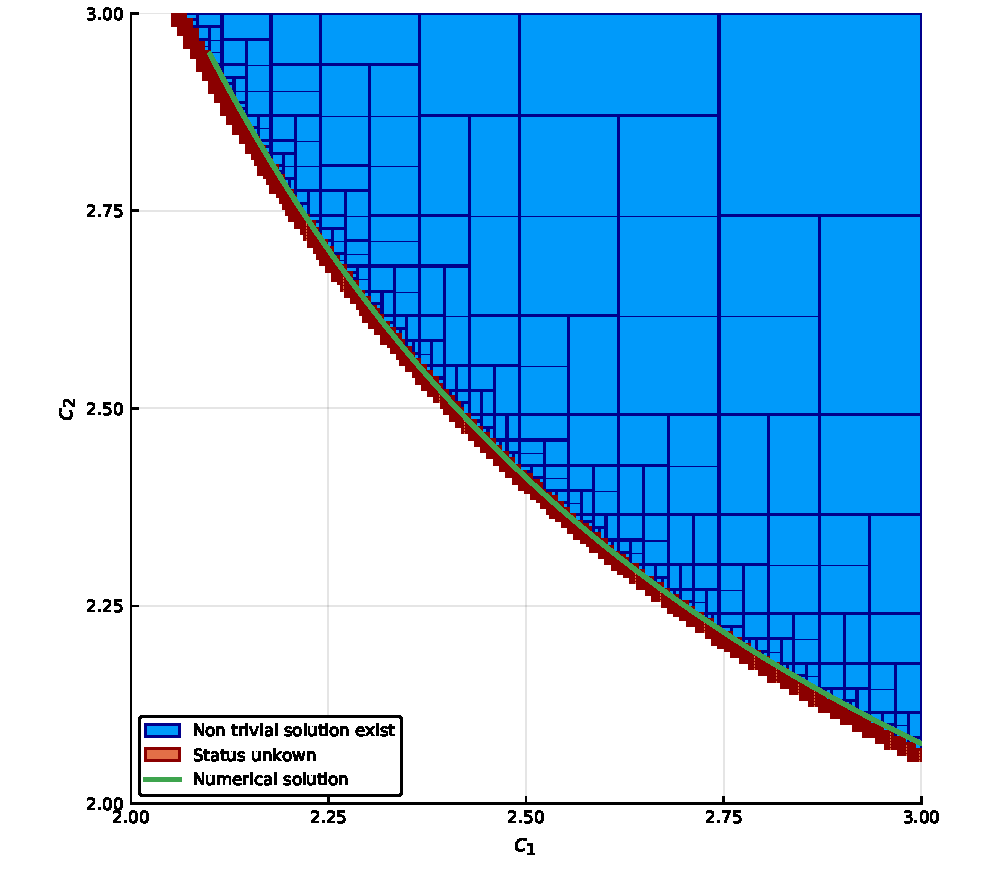
\includegraphics[width=0.8\textwidth]{two_layers_erdos_renyi_boundary.pdf}
	\caption{Phase diagram for a multiplex network composed of two Erdos-Renyi layer with mean degree $c_1$ and $c_2$. In the blue region a non trivial solution for $\uvec$ has been found, in the uncolored region only the trivial solution $\uvec_T$ exists and in the red region the algorithm was unable to conclude in favor of either case. The solid green line is the numerical solution to eq. \eqref{Multiplex u final} and \eqref{Boundary condition}.}
	\label{Figure: Regions and boundary}
	\todo[inline]{Make the plot more readable and less ugly}
	\todo[inline]{Find why the two methods seems drift away one from the other far from the center.}
\end{figure}

%--------------------------------------------
%	THESIS CONTENT - APPENDICES
%--------------------------------------------

\appendix % Cue to tell LaTeX that the following "chapters" are Appendices

\chapter{Fixpoint iteration for connected networks generation}
\section{Convergence of the fixpoint iteration}
\label{Appendix: Fixpoint convergence}

First notice that the case $r_1 = 0$ is trivial, as described in the main text. We will therefore assume in this Appendix that $r_1 > 0$, immediately giving $\mu(0) = r_1 > 0$. Second, not that \eqref{Defition of mu} tells us that $z < 1$ implies $\mu(z) < 1$. From there we separate two cases:

If $u = 1$ is the unique solution of eq. \eqref{Fixpoint equation for u} then $\mu(z)$ must be continuous for $z \in [0, 1]$ and $\mu'(1) < 1$, making $u = 1$ and attractive fixpoint. On the other hand if there is another solution $u^*$ to eq. \eqref{Fixpoint equation for u}, it is the unique solution with $0 \leq u^* < 1$ since $\mu(z)$ is an increasing function of $z$, as it is demonstrated in Appendix \ref{Appendix: Monotonicity}. Moreover, since $\mu(0) > 0$ we have $\mu'(u^*) < 1$, which makes it an attracting fixpoint and makes $u = 1$ a repulsive one.

We can thus conclude that the fixpoint iteration proposed always converges and converges to the degenerate case $u = 1$ only if it is the unique possibility.

\section{Monotonicity of $\mu(z)$}
\label{Appendix: Monotonicity}

To prove that $\mu(z)$ is an increasing function, we compute its derivative with respect to $z$, which yields
\begin{align}
	\mu'(z) &= \left[\sum_{k = 1}^{\infty}k \pi_k(z)\right]^{-2} \left(s_1(z) + s_2(z)\right) \\
	s_1(z) &= \sum_{j, k}k j \pi_k'(z) \pi_j(z) \left( z^{k-1} -  z^{j-1}\right) \\
	s_2(z) &= \sum_{j, k} k (k - 1) j \pi_k(z) \pi_j(z) z^{k-2}.
\end{align}
The sum $s_1(z)$ can be rewritten as
\begin{align}
	s_1(z) &= \sum_{j > k} k j \left(\pi_k'(z) \pi_j(z) - \pi_j'(z) \pi_k(z)\right) \left(z^{k-1} -  z^{j-1}\right) \\
		&=\sum_{j > k} \frac{k r_k}{1 - z^k} \frac{j r_j}{1 - z^j} \frac{z^k - z^j}{z^2} \left(\frac{k}{z^{-k} - 1} - \frac{j}{z^{-j} - 1}\right)\\
		&=\sum_{j > k} k j \pi_k(z) \pi_j(z) \frac{z^k - z^j}{z^2} \left(\frac{k}{z^{-k} - 1} - \frac{j}{z^{-j} - 1}\right).
\end{align}
Using the fact that the function
\begin{align}
	f_z(\lambda) = \frac{\lambda}{z^{-\lambda} - 1}
\end{align}
is a decreasing function of $\lambda$ we can see that for $z \in [0, 1)$ and $j > k$ we have
\begin{align}
	z^k - z^j &\geq 0 \\
	\frac{k}{z^{-k} - 1} - \frac{j}{z^{-j} - 1} &\geq 0,
\end{align}
and thus $s_1(z) \geq 0$. Moreover each terms in $s_2(z)$ is non-negative, so we have $s_2(z) \geq 0$. We can therefore conclude that $\mu'(z) \geq 0$ and thus that $\mu(z)$ is an increasing function of $z$.

%--------------------------------------------
%	BIBLIOGRAPHY
%--------------------------------------------

\printbibliography[heading=bibintoc]{}

% \printindex{}

\end{document}